% \documentclass[aspectratio=169,onlytextwidth,english]{beamer}
\documentclass[onlytextwidth,english]{beamer}\usepackage[]{graphicx}\usepackage[]{xcolor}
% maxwidth is the original width if it is less than linewidth
% otherwise use linewidth (to make sure the graphics do not exceed the margin)
\makeatletter
\def\maxwidth{ %
  \ifdim\Gin@nat@width>\linewidth
    \linewidth
  \else
    \Gin@nat@width
  \fi
}
\makeatother

\definecolor{fgcolor}{rgb}{0.345, 0.345, 0.345}
\newcommand{\hlnum}[1]{\textcolor[rgb]{0.686,0.059,0.569}{#1}}%
\newcommand{\hlsng}[1]{\textcolor[rgb]{0.192,0.494,0.8}{#1}}%
\newcommand{\hlcom}[1]{\textcolor[rgb]{0.678,0.584,0.686}{\textit{#1}}}%
\newcommand{\hlopt}[1]{\textcolor[rgb]{0,0,0}{#1}}%
\newcommand{\hldef}[1]{\textcolor[rgb]{0.345,0.345,0.345}{#1}}%
\newcommand{\hlkwa}[1]{\textcolor[rgb]{0.161,0.373,0.58}{\textbf{#1}}}%
\newcommand{\hlkwb}[1]{\textcolor[rgb]{0.69,0.353,0.396}{#1}}%
\newcommand{\hlkwc}[1]{\textcolor[rgb]{0.333,0.667,0.333}{#1}}%
\newcommand{\hlkwd}[1]{\textcolor[rgb]{0.737,0.353,0.396}{\textbf{#1}}}%
\let\hlipl\hlkwb

\usepackage{framed}
\makeatletter
\newenvironment{kframe}{%
 \def\at@end@of@kframe{}%
 \ifinner\ifhmode%
  \def\at@end@of@kframe{\end{minipage}}%
  \begin{minipage}{\columnwidth}%
 \fi\fi%
 \def\FrameCommand##1{\hskip\@totalleftmargin \hskip-\fboxsep
 \colorbox{shadecolor}{##1}\hskip-\fboxsep
     % There is no \\@totalrightmargin, so:
     \hskip-\linewidth \hskip-\@totalleftmargin \hskip\columnwidth}%
 \MakeFramed {\advance\hsize-\width
   \@totalleftmargin\z@ \linewidth\hsize
   \@setminipage}}%
 {\par\unskip\endMakeFramed%
 \at@end@of@kframe}
\makeatother

\definecolor{shadecolor}{rgb}{.97, .97, .97}
\definecolor{messagecolor}{rgb}{0, 0, 0}
\definecolor{warningcolor}{rgb}{1, 0, 1}
\definecolor{errorcolor}{rgb}{1, 0, 0}
\newenvironment{knitrout}{}{} % an empty environment to be redefined in TeX

\usepackage{alltt}

% use official beamer theme from uzh
\usetheme[english]{uzh} 

% First installation of languages required
% tinytex::tlmgr_install("babel-english")
% tinytex::tlmgr_install("babel-german")


%% load relevant packages:


\usepackage[T1]{fontenc}
\usepackage[latin9]{inputenc}
%\usepackage[english]{babel}
\usepackage{pgfpages}           % necessary for the handouts production
\usepackage{amsmath}            % for nice mathematics
\usepackage{verbatim}           % for verbatim output
\usepackage{wasysym}            % symbols (smilies etc.)
\usepackage{longtable}
\usepackage{float}
\usepackage{textcomp}
\usepackage{graphicx}
\usepackage{xcolor} % for the color names, see: http://en.wikibooks.org/wiki/LaTeX/Colors#Predefined_
\usepackage{natbib}             % for bibliography style and citations
\usepackage{hyperref}
\usepackage{caption}
\hypersetup{%
    hyperindex=true,
    colorlinks=true,%
    urlcolor = {uzh@blue},% in theme uzh
    citecolor = {uzh@blue},
    urlcolor = {uzh@berry},
    pdfstartview=Fit,%
    pdfpagelayout=SinglePage,%
    pdfpagemode=UseThumbs
  }%
\usepackage{url}
\DeclareOptionBeamer{compress}{\beamer@compresstrue}
\ProcessOptionsBeamer

%% define slidetitle color
\setbeamercolor{title}{fg=uzh@blue}
\setbeamercolor{frametitle}{fg=uzh@blue}


% \title{Neural Causal Models with TRAM-DAGs}
\title{\normalsize Modeling Functional Relationships in Causal Graphs and Estimating Individualized Interventions: Neural Causal Models (TRAM-DAGs) and Conditional Average Treatment Effects}


%% The following are all optional, simply comment them
%\subtitle{Subtitle (optional)}
\institute{Master Program in Biostatistics www.biostat.uzh.ch\\ Master Thesis: Final Presentation}  %% optional
% leave some vertical space here

\author{Mike Kr{\"a}henb{\"u}hl, Supervisors: Beate Sick, Oliver D{\"u}rr }
\date{\today}
\titlegraphic{img/uzh-lake.jpg}


%%%%%%%%%%%%%%%%%%%%%%%%%%%%%%%%%%%%%%%%%%%%%%%%%%%%%%%% 


\IfFileExists{upquote.sty}{\usepackage{upquote}}{}
\begin{document}

\maketitle



% 
% \begin{frame}{Background}
% 
% \begin{columns}
% 
% % Left side: Text (approx. 3/4 of the slide)
% \begin{column}{0.7\textwidth}
% \textbf{Supervisors:}
% \begin{itemize}
%     \item Beate Sick, UZH
%     \item Oliver D{\"u}rr, HTWG Konstanz
% \end{itemize}
% 
% \textbf{Paper \textit{"Interpretable Neural Causal Models with TRAM-DAGs"} \citep{sick2025}:}
% \begin{itemize}
%     \item Framework to model causal relationships
%     \item Based on transformation models
%     \item Rely on (deep) neural networks
%     \item Compromise between interpretability and flexibility
% \end{itemize}
% \end{column}
% 
% % Right side: Image (approx. 1/4 of the slide)
% \begin{column}{0.3\textwidth}
% 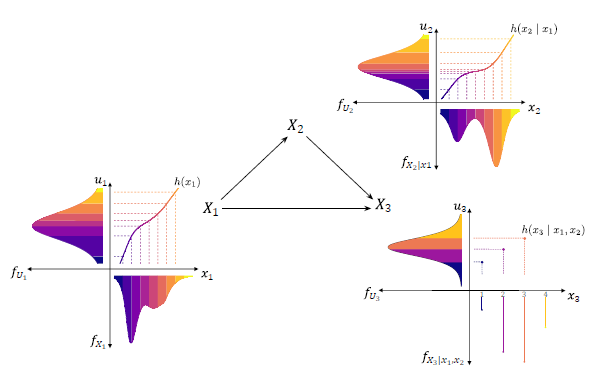
\includegraphics[width=\textwidth]{img/TRAM_DAG_Background.png}
% \end{column}
% 
% \end{columns}
% 
% \end{frame}
% 
% 
% 
% 
% 
% 
% 
% 
% 
% 
% 
% 
% \begin{frame}{Individualized Treatment Effect (ITE)}
% 
% 
% ITE Estimation formula and assumptions
% 
% how heterogeneity happens
% 
% \end{frame}
% 
% 
% 
% \begin{frame}{Causal ML Models for ITE estimation}
% 
% Meta learners (T-learner, S-learner etc.)
% 
% 
% Tram dags
% 
% \end{frame}
% 
% 
% 
% 
% 
% \begin{frame}{IST Stroke trial}
% 
% 
% Explain the trial
% 
% \end{frame}
% 
% 
% 
% 
% 
% 
% \begin{frame}{IST Stroke trial: Results with GLM}
% 
% Show results of tlearner GLM
% 
% \end{frame}
% 
% 
% \begin{frame}{IST Stroke trial: Results with Random Forest}
% 
% 
% 
% 
% 
% 
% 
% 
% \end{frame}
% 
% 
% \begin{frame}{IST Stroke trial: Results with tram dag}
% 
% Show results of tram dag
% 
% \end{frame}
% 
% 
% 
% \begin{frame}{Simulation: When do problems occur?}
% 
% explain setup with dag and effect sizes and interactions that affect outcome
% 
% \end{frame}
% 
% 




\begin{frame}{Simulation Case 1: Fully Observed}

\begin{columns}

% Left column: Text
\begin{column}{0.52\textwidth}

\vspace{-0.5em}
\textbf{Setup:}
\begin{itemize}\setlength\itemsep{0.4em}
  \item $n = 20{,}000$
  \item $T \sim \text{Bernoulli}(0.5)$
  \item $\mathbf{X} = (X_1, \dots, X_5)^\top \sim \mathcal{N}(\mathbf{0}, \Sigma)$\\
  \item $\mathbf{X_{TX}} = (X_1, X_2)^\top$ \textcolor{red}{interaction}
\end{itemize}


\end{column}

% Right column: DAG image
\begin{column}{0.42\textwidth}
    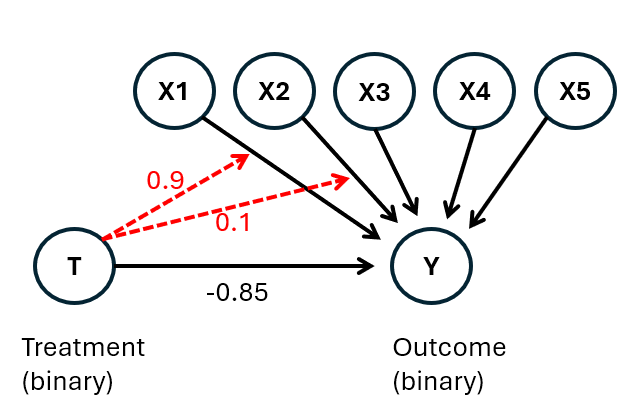
\includegraphics[width=\textwidth]{img/simulation_observed.png}
\end{column}

\end{columns}


\vspace{0.3em}
\textbf{Outcome model:}
\[
\mathbb{P}(Y = 1 \mid \mathbf{X}, T) = \text{logit}^{-1} \left(
\beta_0 + \beta_T T + \boldsymbol{\beta}_X^\top \mathbf{X}
+ \textcolor{red}{T \cdot \boldsymbol{\beta}_{TX}^\top \mathbf{X_{TX}}}
\right)
\]


\end{frame}





\begin{frame}{Simulation Case 1: Fully Observed}

Results with T-learner logistic regression (glm):

% Below: image
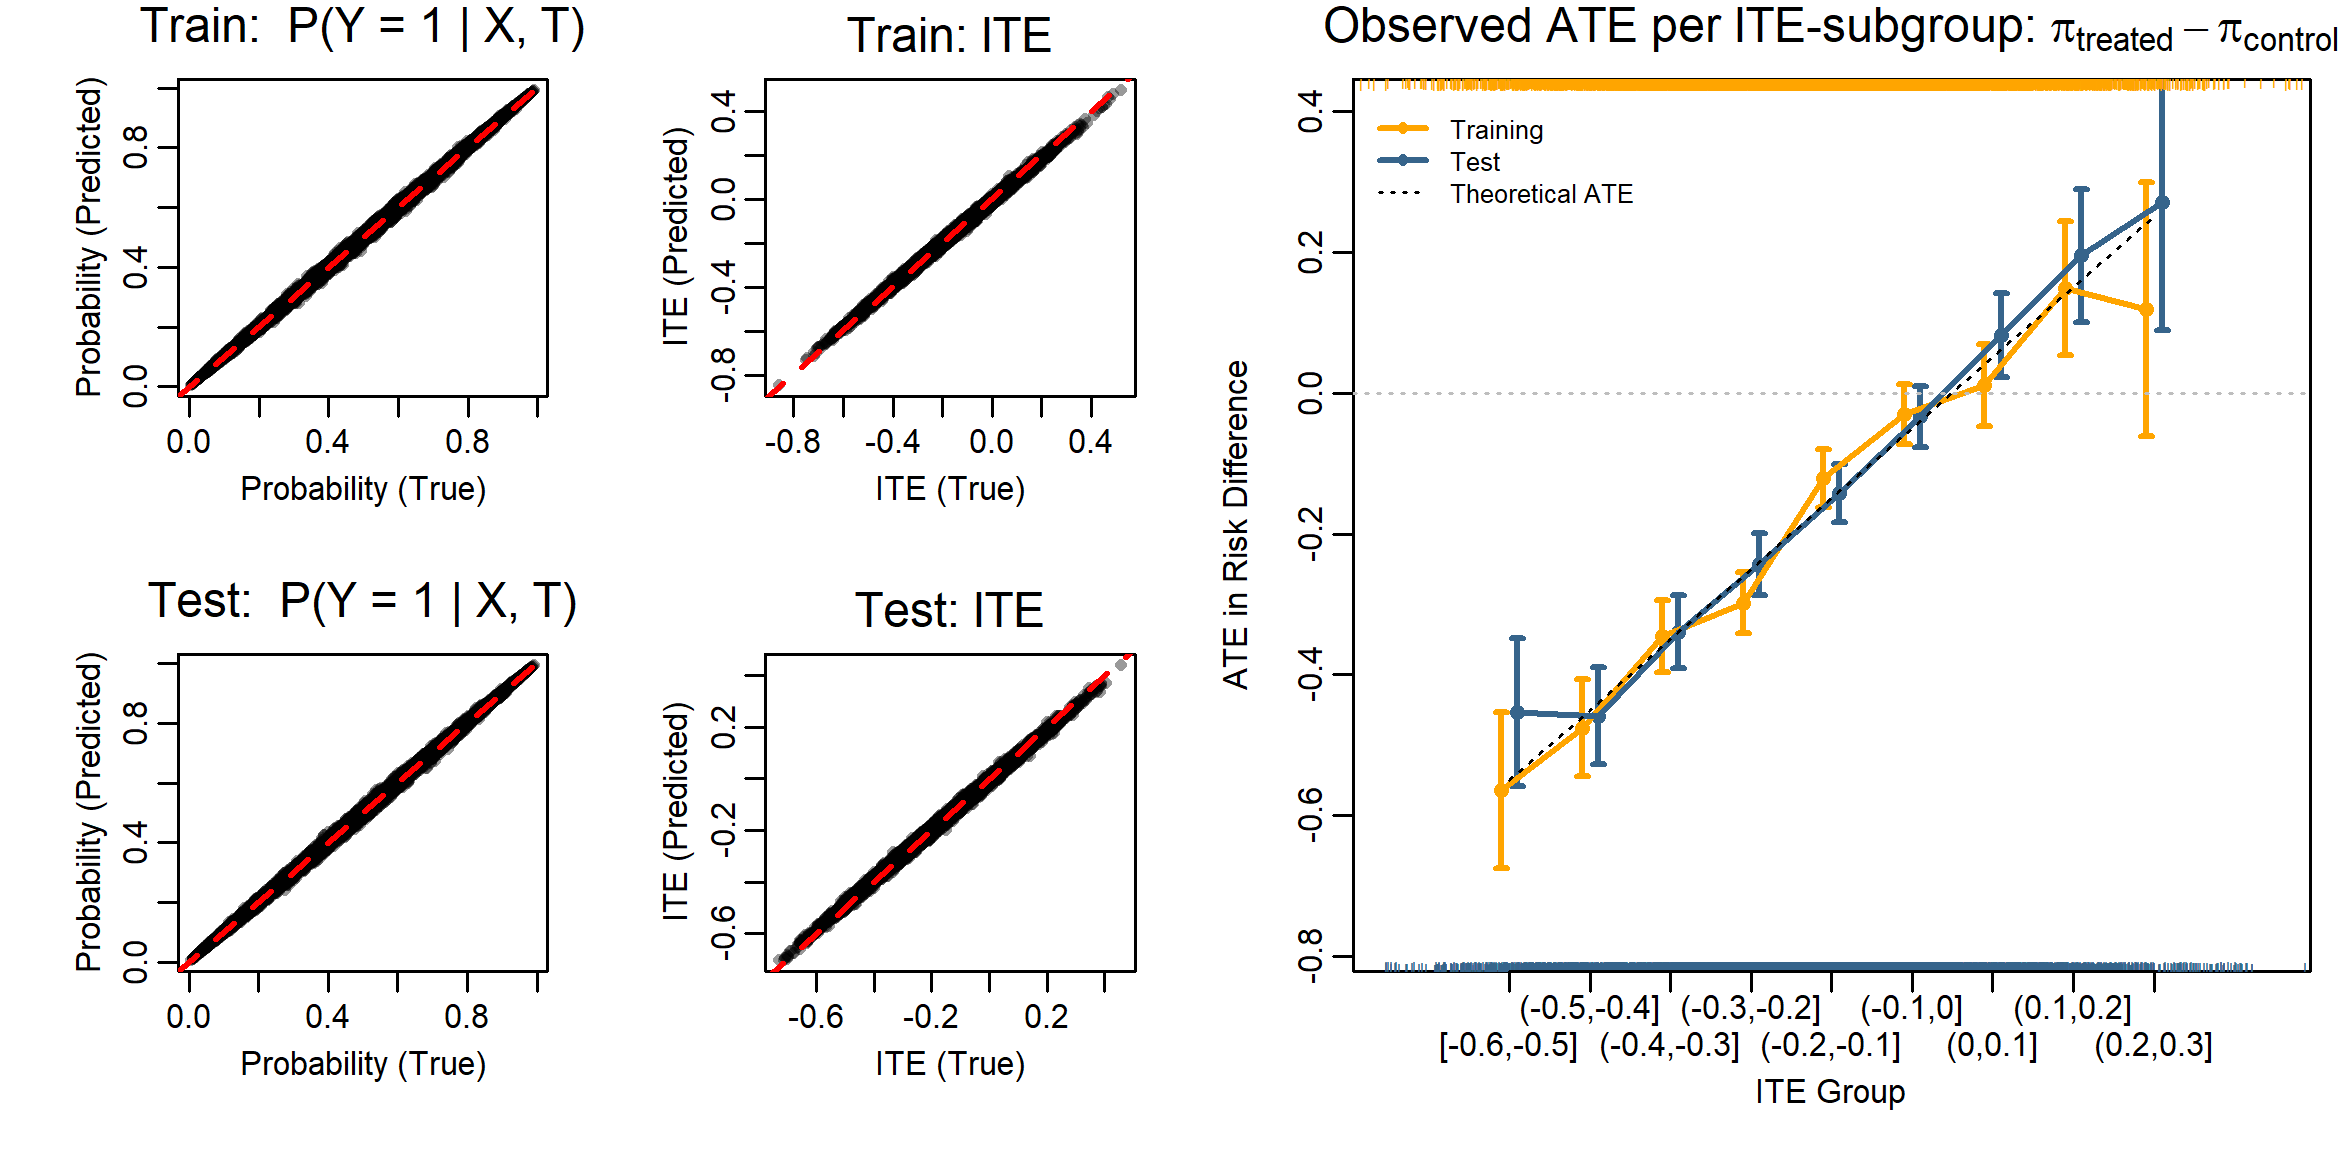
\includegraphics[width=\textwidth]{img/fully_observed_glm_tlearner.png}

\end{frame}


\begin{frame}{Simulation Case 1: Fully Observed}

Results with T-learner Random Forest (comets package):

% Below: image
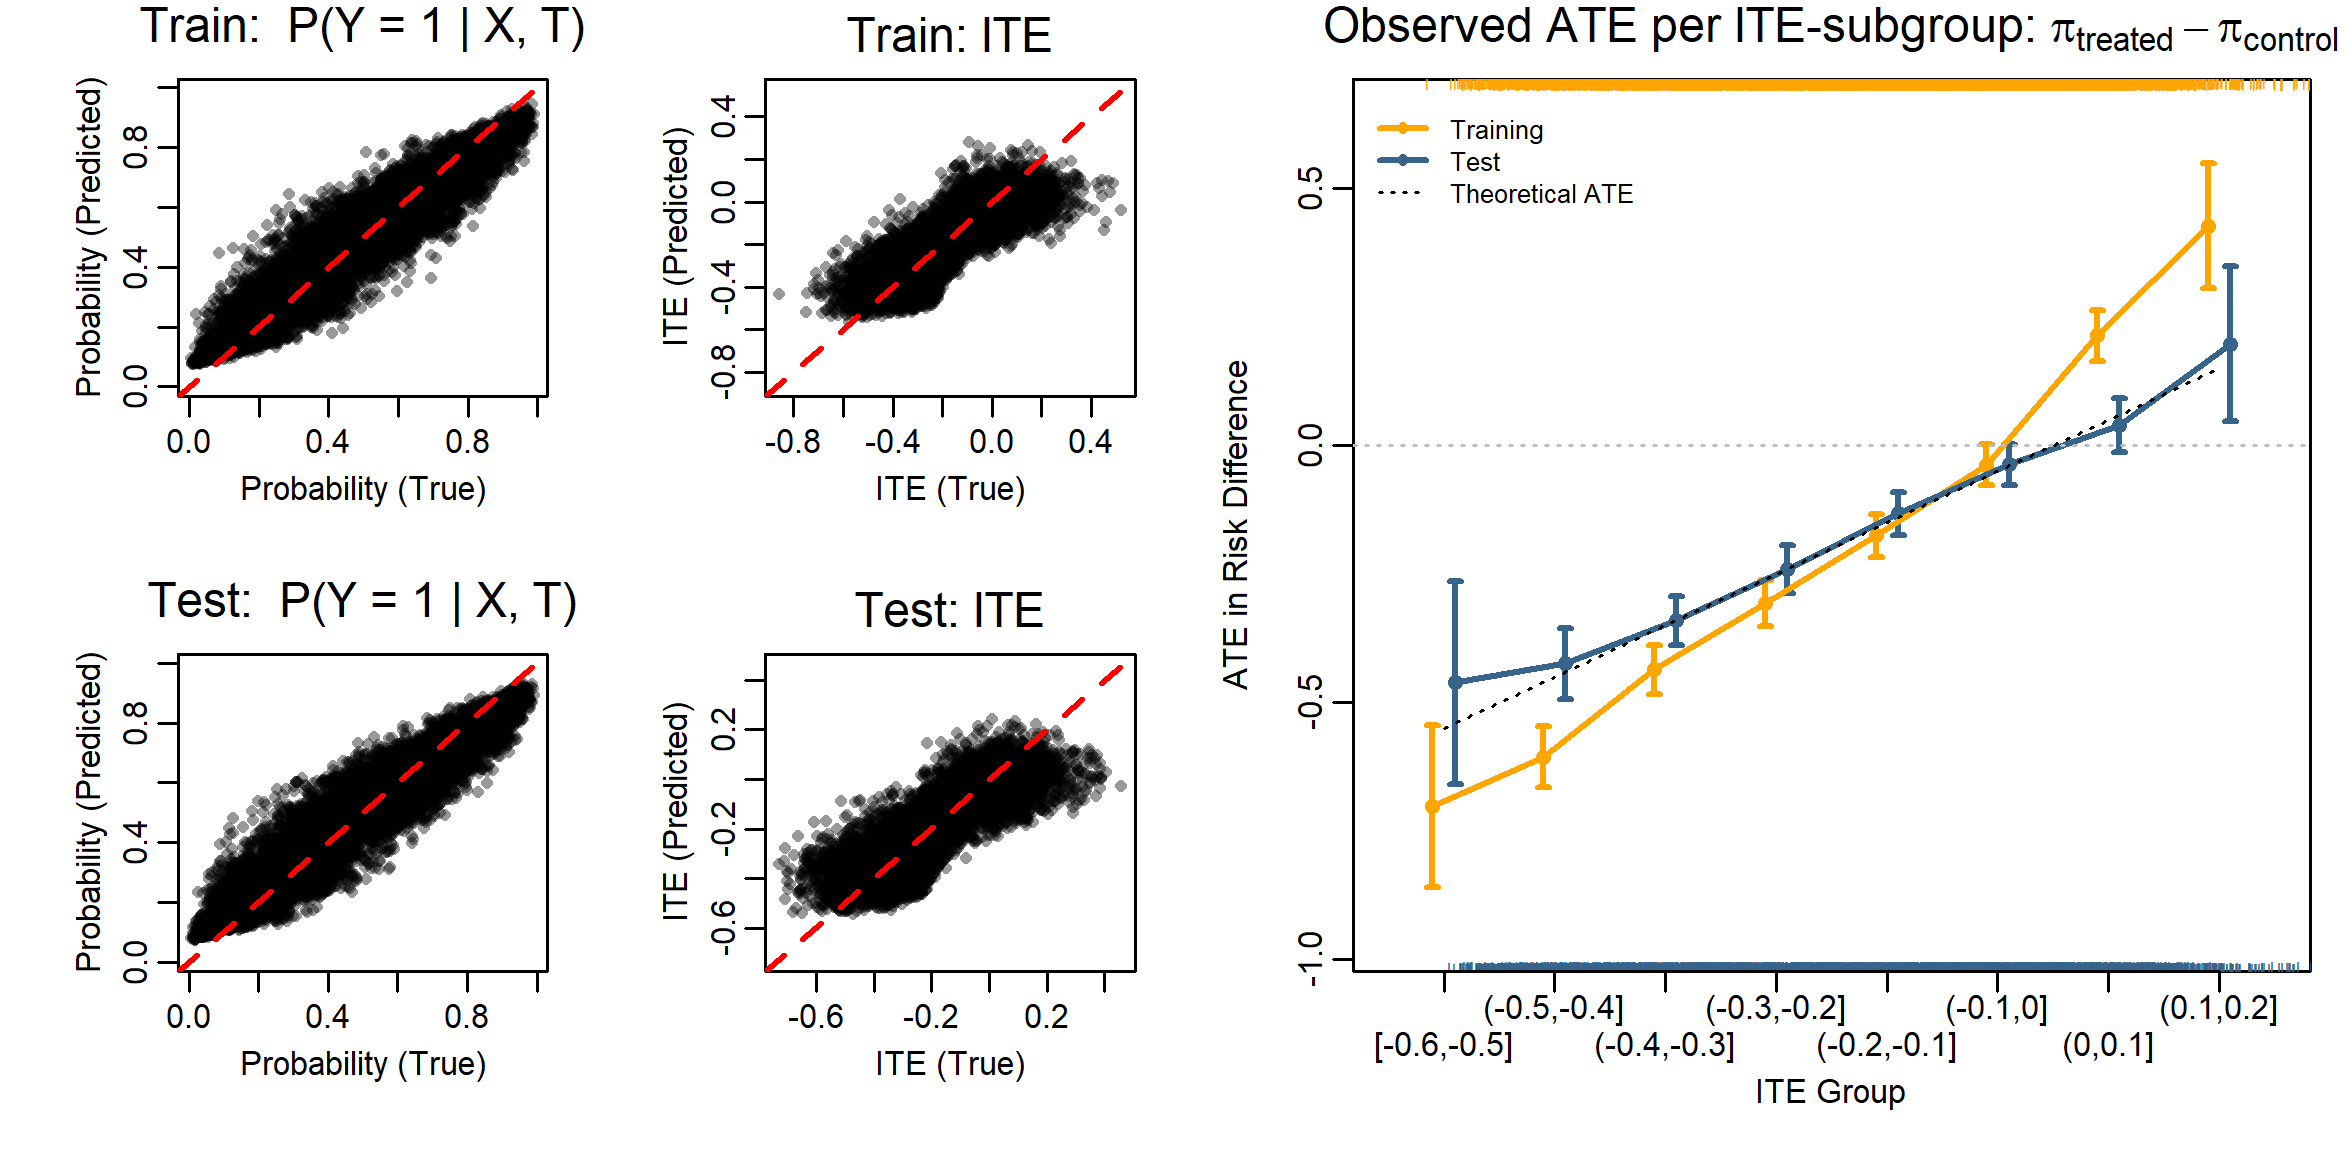
\includegraphics[width=\textwidth]{img/observed_tuned_rf.png}

\end{frame}







\begin{frame}{Simulation Case 2: Unobserved Interaction}

\begin{columns}

% Left column: Text
\begin{column}{0.52\textwidth}

\vspace{-0.5em}
\textbf{Setup:}
\begin{itemize}\setlength\itemsep{0.4em}
  \item $n = 20{,}000$
  \item $T \sim \text{Bernoulli}(0.5)$
  \item $\mathbf{X} = (X_1, \dots, X_5)^\top \sim \mathcal{N}(\mathbf{0}, \Sigma)$\\
  \item $\mathbf{X_{TX}} = (X_1, X_2)^\top$ \textcolor{red}{interaction}
\end{itemize}


\end{column}

% Right column: DAG image
\begin{column}{0.42\textwidth}
    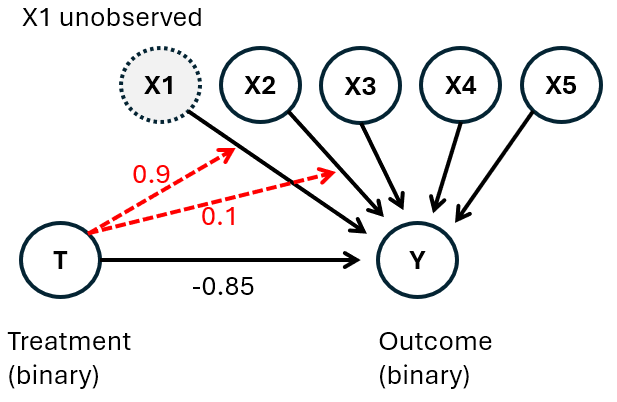
\includegraphics[width=\textwidth]{img/simulation_unobserved.png}
\end{column}

\end{columns}


\vspace{0.3em}
\textbf{Outcome model:}
\[
\mathbb{P}(Y = 1 \mid \mathbf{X}, T) = \text{logit}^{-1} \left(
\beta_0 + \beta_T T + \boldsymbol{\beta}_X^\top \mathbf{X}
+ \textcolor{red}{T \cdot \boldsymbol{\beta}_{TX}^\top \mathbf{X_{TX}}}
\right)
\]

% in this scenario X1 is unobserved
\textbf{Note:} Same DGP, but $X_1$ is not observed!

\end{frame}




\begin{frame}{Simulation Case 2: Unobserved Interaction}

Results with T-learner logistic regression (glm):

% Below: image
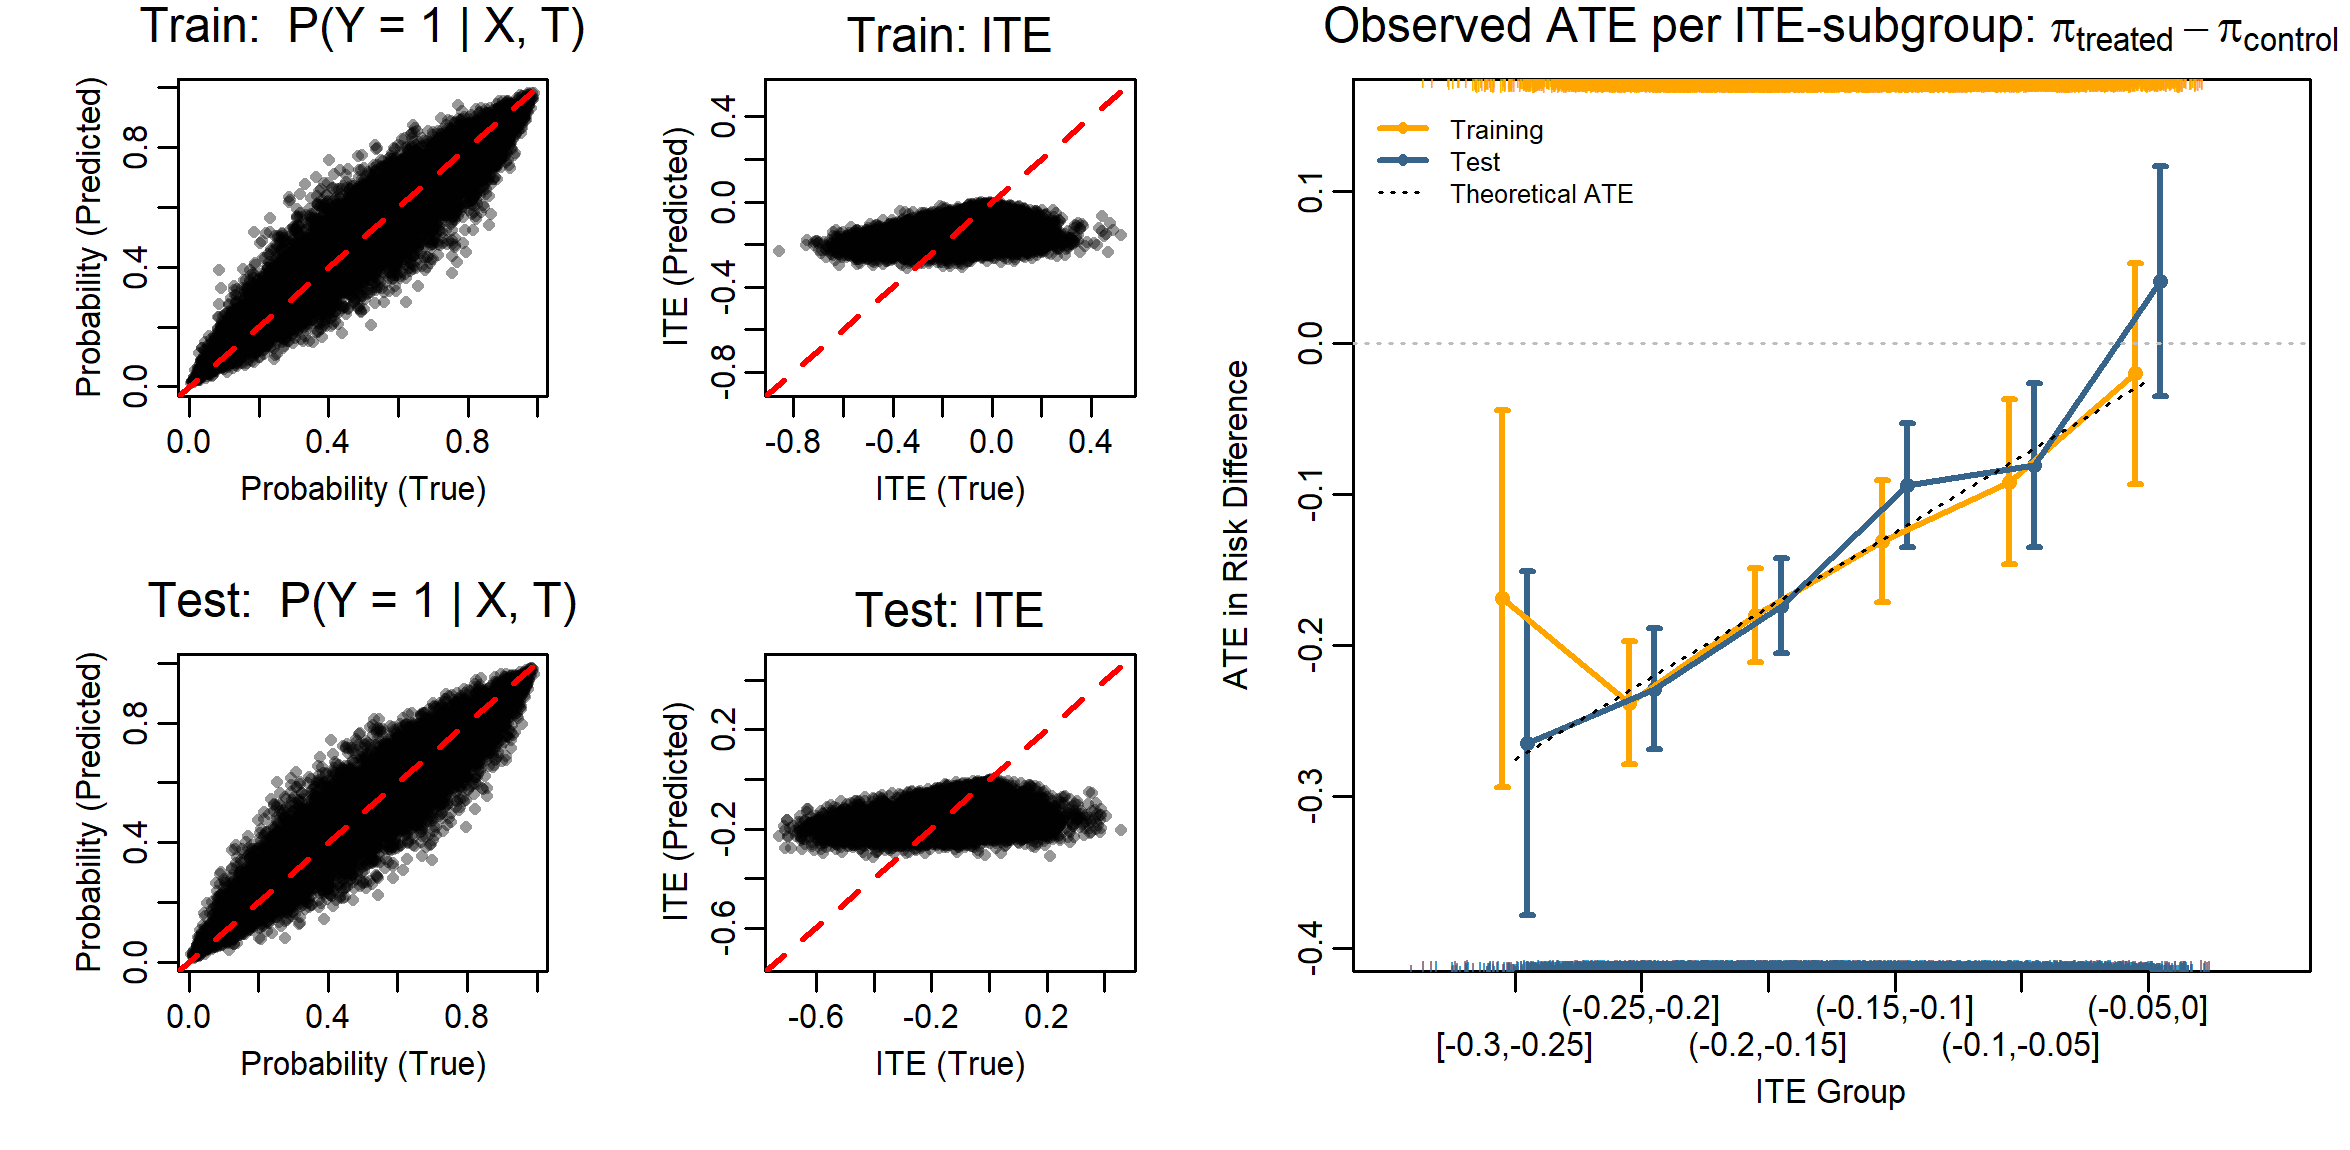
\includegraphics[width=\textwidth]{img/unobserved_interaction_glm_tlearner.png}

\end{frame}

\begin{frame}{Simulation Case 2: Unobserved Interaction}

Results with T-learner Random Forest (comets):

% Below: image
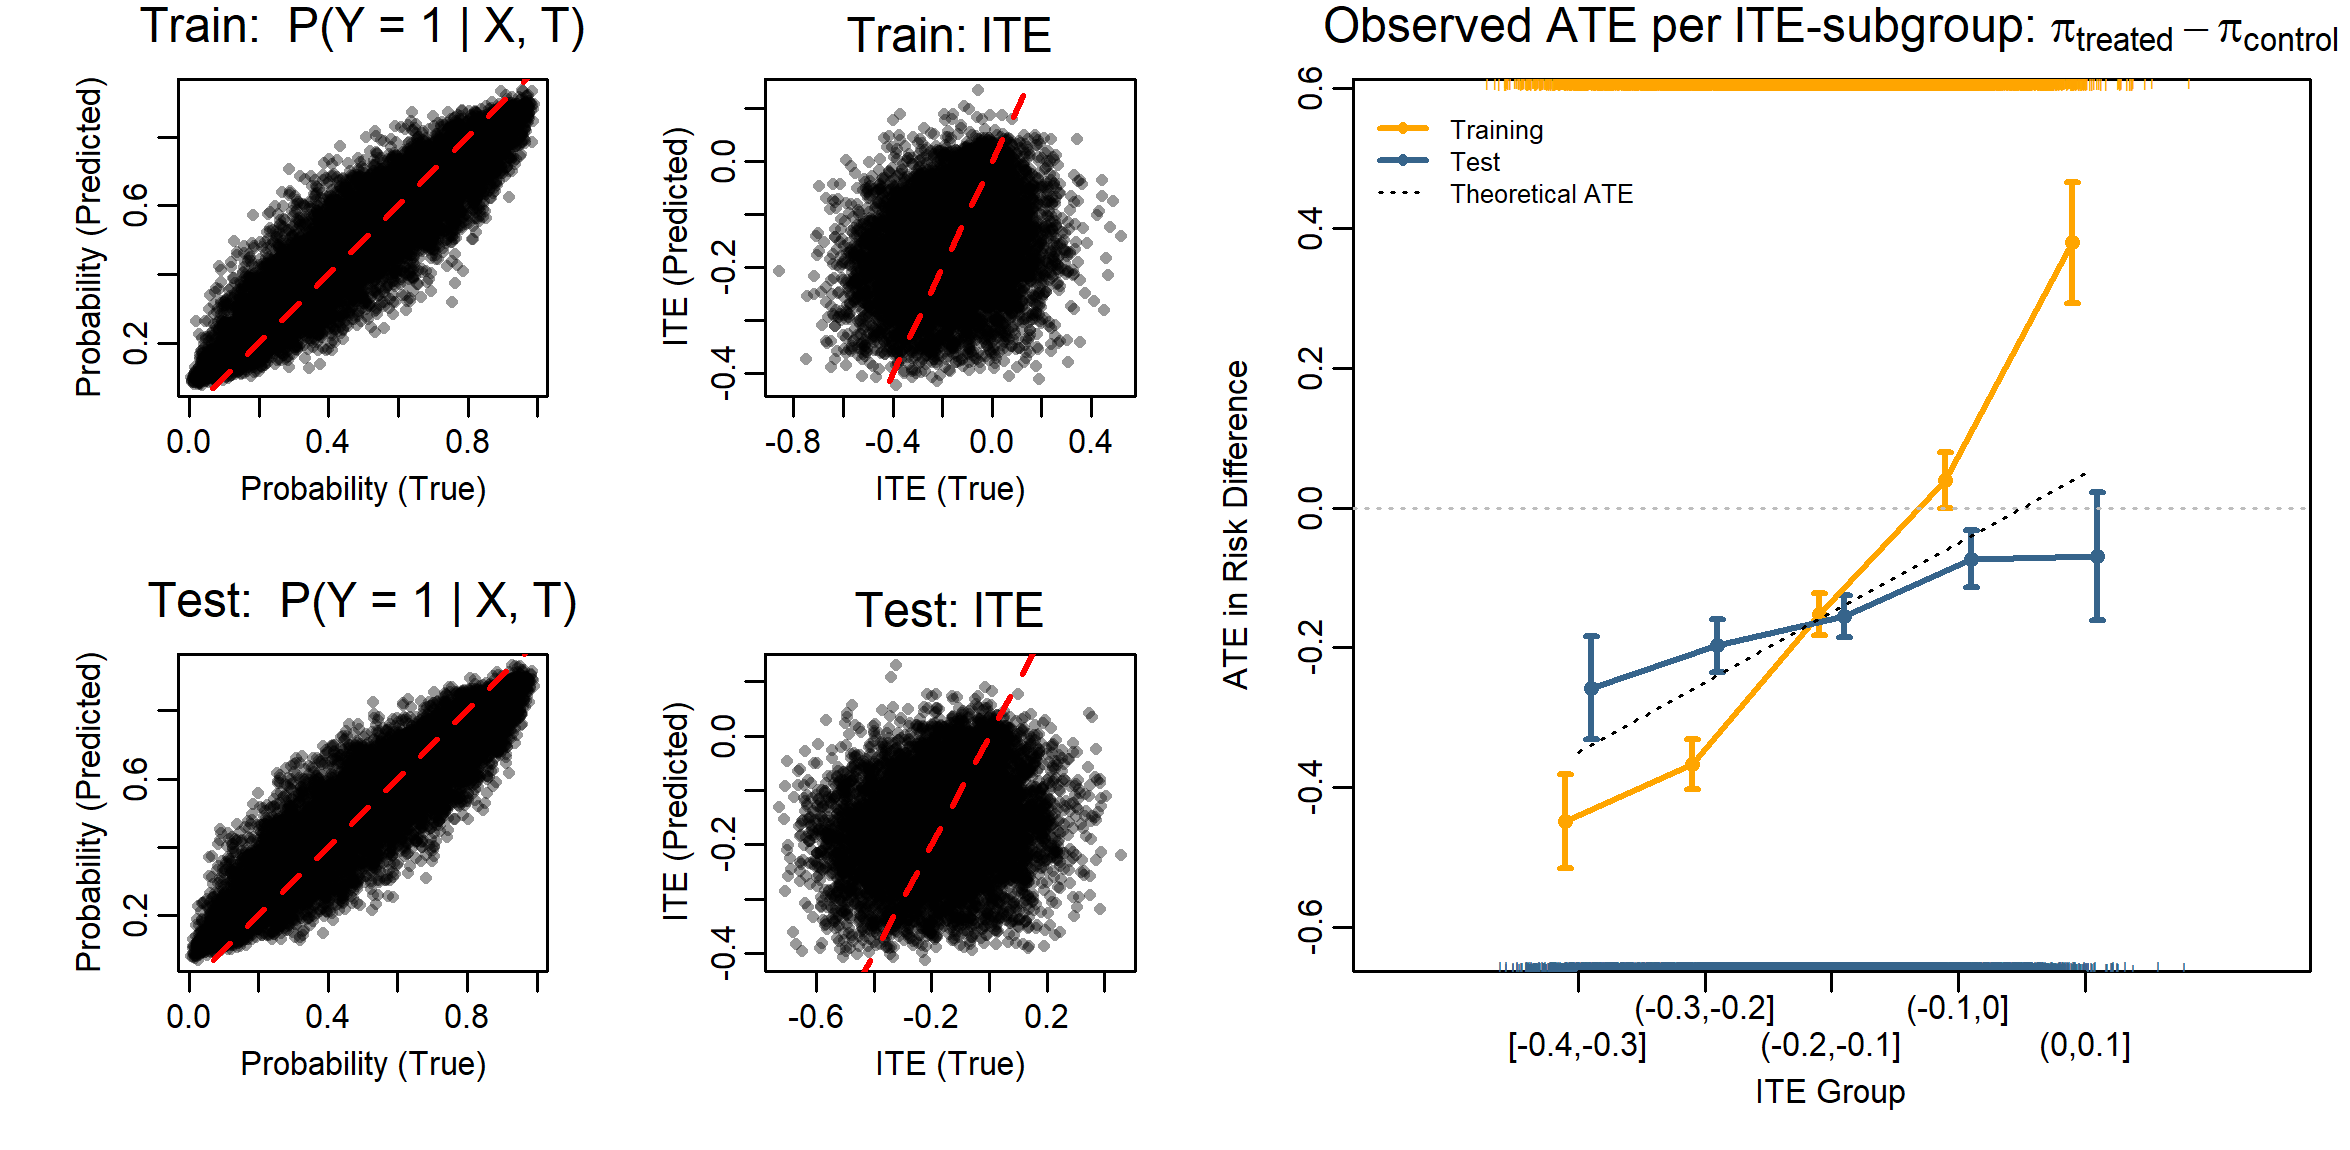
\includegraphics[width=\textwidth]{img/unobserved_tuned_rf.png}

\end{frame}






\begin{frame}{Simulation Case 2: Unobserved Interaction III}

\textbf{My interpretation:} 
\begin{itemize}
    \item When a high predicted treatment effect (ITE) corresponds to a high observed effect in the train set (strong discrimination), but not in the test set, it might be due to unobserved interaction variables.
    \item This is more likely to occur with complex models, as they tend to overfit when the interaction is not observed.
    % as they tend to predict a wider range of ITEs than simpler models
\end{itemize}


\end{frame}





\begin{frame}{TRAM-DAGs for ITE Estimation}

\begin{columns}

% Left side: Text (approx. 3/4 of the slide)
\begin{column}{0.7\textwidth}

\textbf{Paper \textit{"Interpretable Neural Causal Models with TRAM-DAGs"} \citep{sick2025}:}
\begin{itemize}
    \item Framework to model causal relationships
    \item Based on transformation models
    \item Rely on (deep) neural networks
    \item Compromise between interpretability and flexibility
\end{itemize}

\textbf{Our Claim:} We can use TRAM-DAGs for ITE estimation, as long as the DAG is known and fully observed!

\end{column}

% Right side: Image (approx. 1/4 of the slide)
\begin{column}{0.3\textwidth}
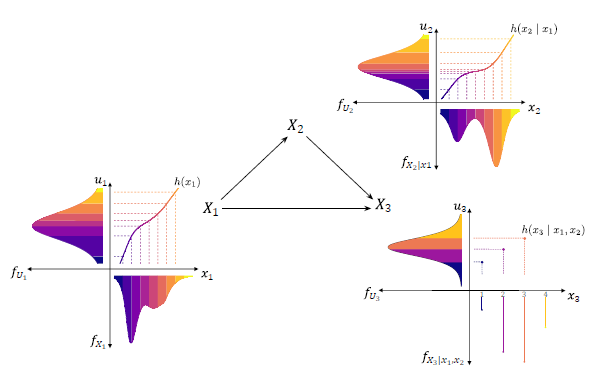
\includegraphics[width=\textwidth]{img/TRAM_DAG_Background.png}
\end{column}

\end{columns}

\end{frame}





\begin{frame}{TRAM-DAGs: Structural Equations}


TRAM-DAGs estimate the structural equations with transformation functions $h_i$:

\begin{columns}

% Left side: Text
\begin{column}{0.5\textwidth}

$Z_i = h_i(X_i \mid \text{pa}(X_i))$ \\
$X_i = h_i^{-1}(Z_i, \text{pa}(X_i)) = f_i(Z_i, \text{pa}(X_i))$ \\

%empty line
\vspace{1.5em}

\begin{itemize}
    \item $\text{pa}(X_i)$: causal parents of $X_i$
    \item $Z_i$: noise distribution (e.g. standard logistic)
\end{itemize}

\end{column}

% Right side: Image
\begin{column}{0.5\textwidth}
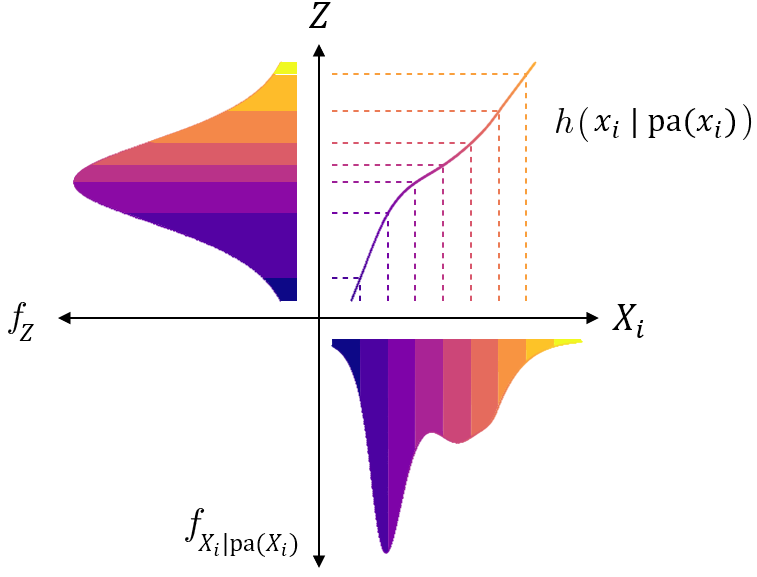
\includegraphics[width=\textwidth]{img/trafo_xi.png}
\end{column}
\end{columns}


\end{frame}





\begin{frame}{TRAM-DAGs: Example for ITE estimation}

\centering
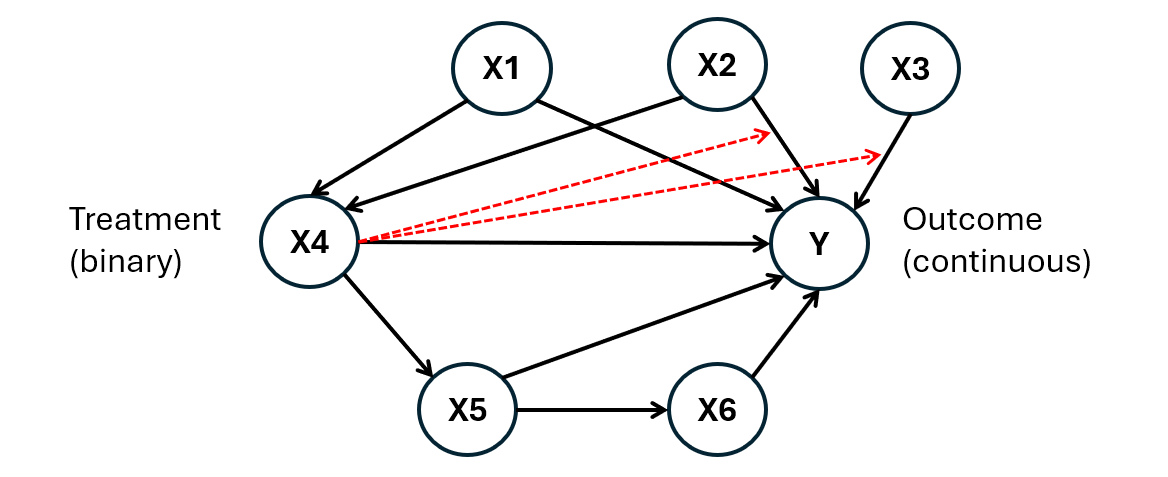
\includegraphics[width=0.8\textwidth]{img/dag_ITE_observational.png}
\normalsize

\vspace{1em} % optional spacing
\raggedright % <--- Ends centering and left-aligns following text

\small
\textbf{DGP:}
\begin{itemize}
    \item $X5 = h_5^{-1}(\epsilon - 0.8 \, X4 )$ \hspace{1em} $\rightarrow$ (depends on treatment)
    \item $X6 = h_5^{-1}(\epsilon + 0.5 \, X5)$ \hspace{1em} $\rightarrow$ (depends on treatment through X5)
    \item $Y = h_6^{-1}(\epsilon - \beta_1 X1 - \beta_2 X2 - \beta_3 X3 - \beta_4 X4 - \beta_5 X5 - \beta_6 X6 - \textcolor{red}{Tr \cdot (\beta_{2Tr} X2 + \beta_{3Tr} X3)})$
\end{itemize}

\end{frame}





\begin{frame}{TRAM-DAGs: Example for ITE estimation}



\[
\text{ITE} = \operatorname{median}(Y \mid \text{do}(T = 1), X) - \operatorname{median}(Y \mid \text{do}(T = 0), X)
\]

\centering

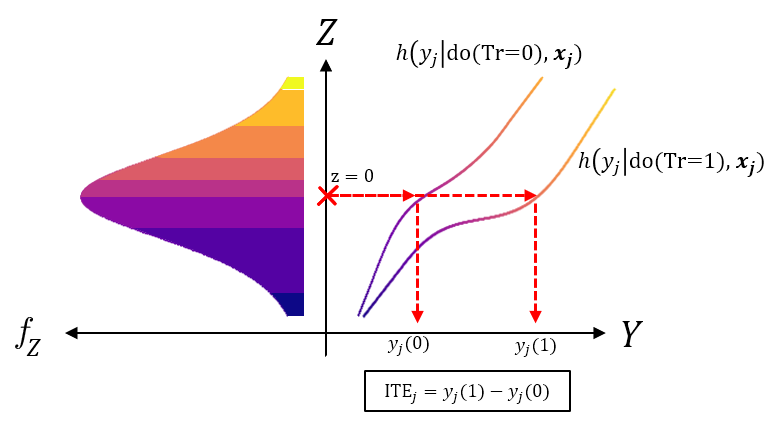
\includegraphics[width=0.7\textwidth]{img/potential_outcomes_y.png}



\end{frame}





\begin{frame}{TRAM-DAGs: Example for ITE estimation}

\[
\text{ITE} = \operatorname{median}(Y \mid \text{do}(T = 1), X) - \operatorname{median}(Y \mid \text{do}(T = 0), X)
\]

\centering
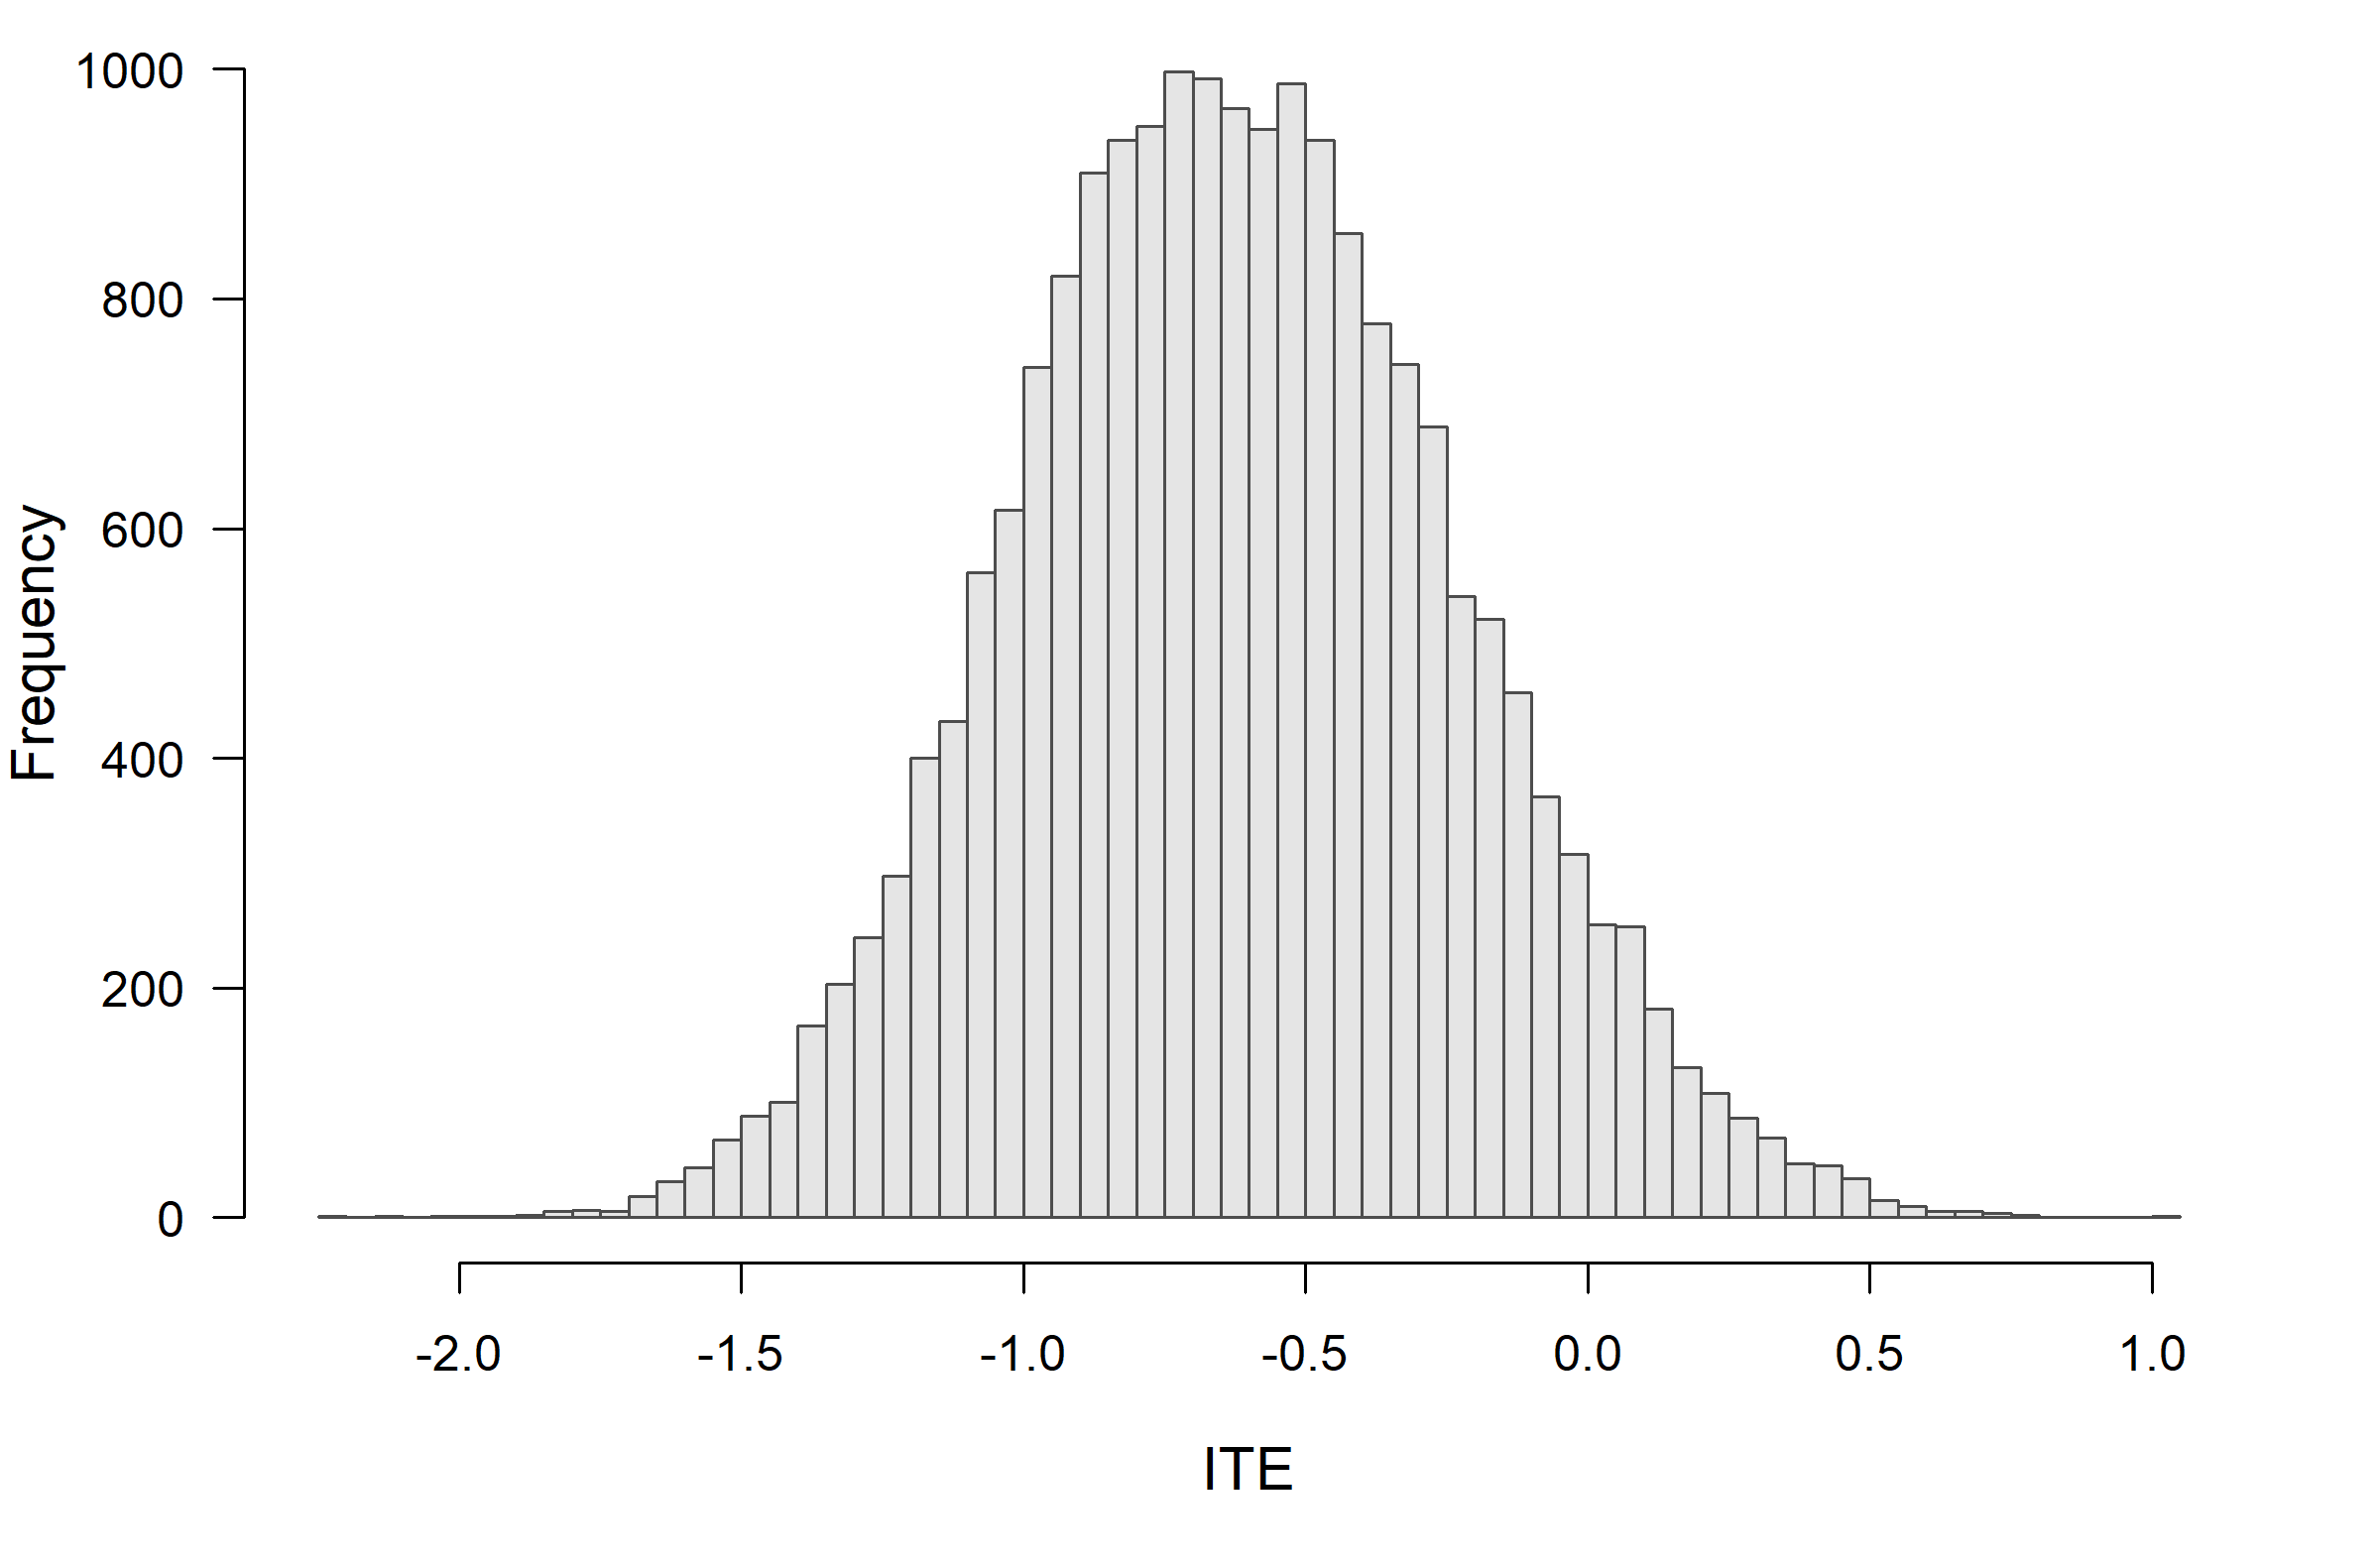
\includegraphics[width=0.7\textwidth]{img/observ_scenario1_ite_distribution_dgp.png}

\end{frame}



\begin{frame}{TRAM-DAGs: Estimate Potential Outcomes II}


\begin{enumerate}
    \item Estimate each $h_i(X_i \mid \text{pa}(X_i)$ fully flexible (deep-NN / complex intercept)
    \item Take the train set or a test set
    \item $Z_i = h(X_i \mid pa(X_i))$ gives us the (observed) latent variable for each $X_i$
    \item Determine counterfactuals for X5 and X6 with the (observed) latent variables $Z_i$
    \item Determine medians of potential outcomes $Y(1)$ and $Y(0)$
    \item $\text{ITE} = \text{median}(Y(1) \mid X_{tx}) - \text{median}(Y(0) \mid X_{ct})$
\end{enumerate}

\end{frame}



\begin{frame}{TRAM-DAGs: Example for ITE estimation (Results)}


\centering
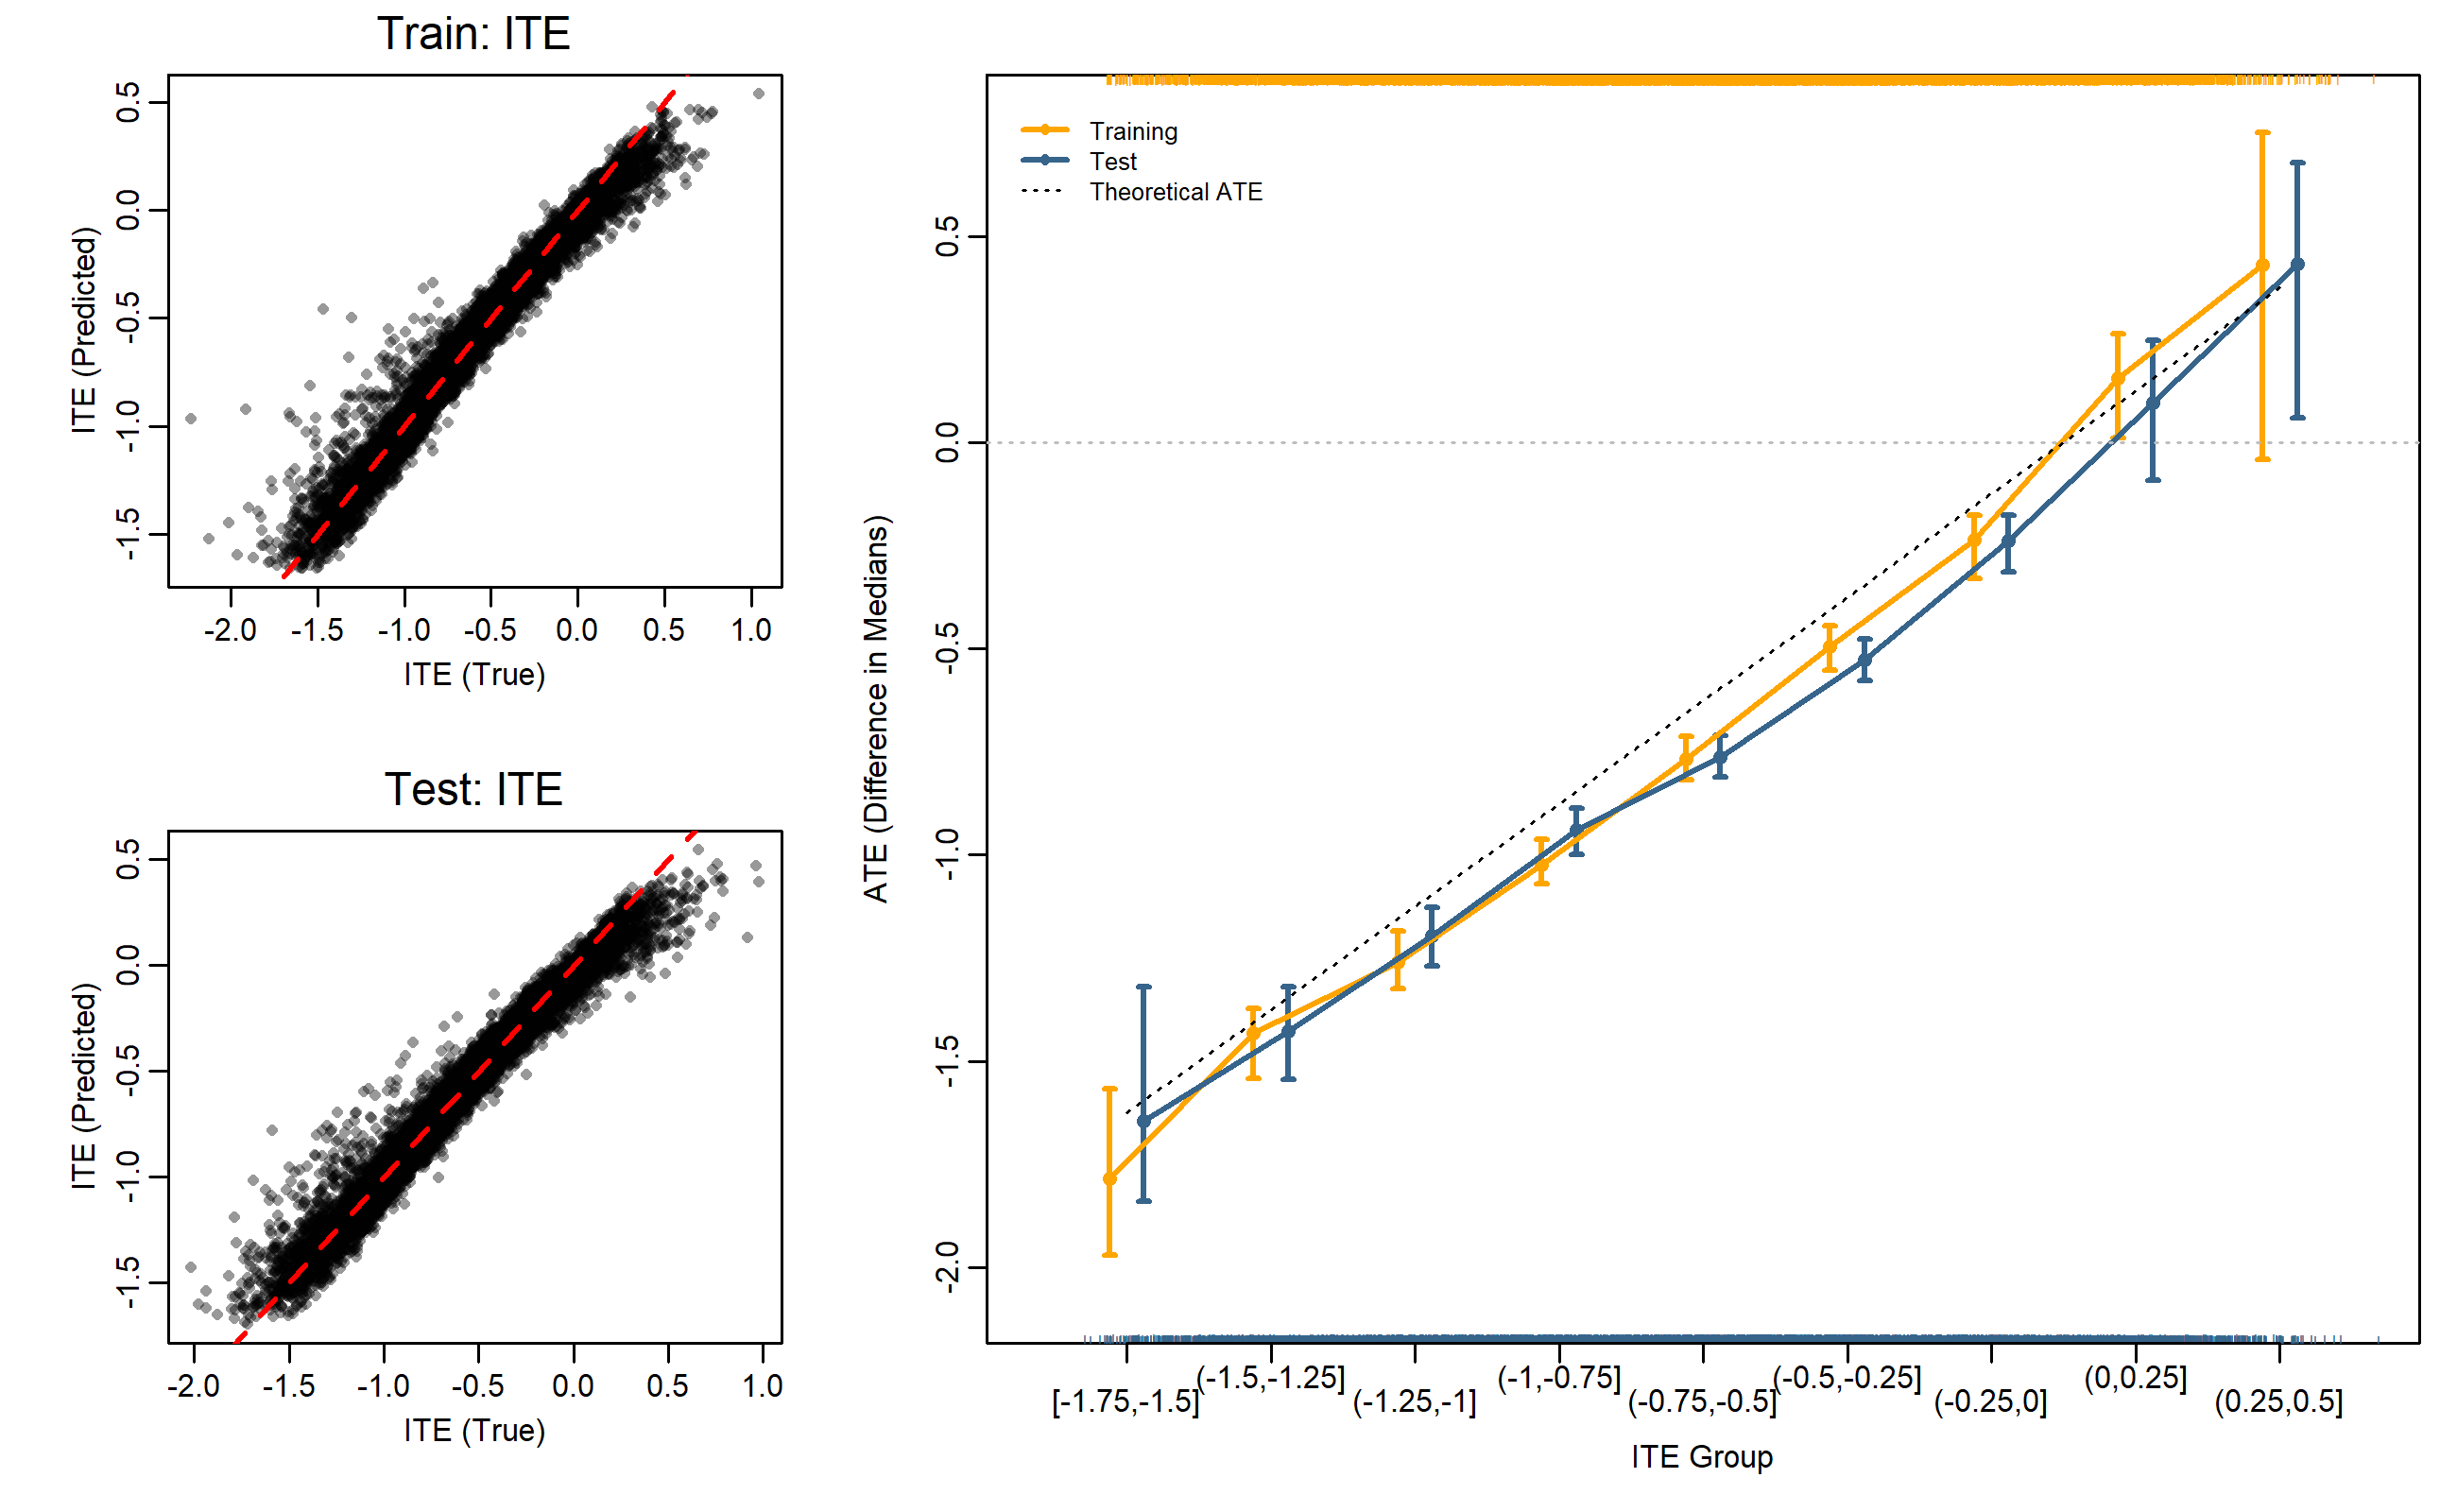
\includegraphics[width=0.9\textwidth]{img/observedITE_ATE_base.png}


\end{frame}




\begin{frame}{TRAM-DAGs: Example for ITE estimation (Results)}



% Comparison of ATE in RCT with $\E(\text{ITE}_{predicted})$


\textbf{ATE TRAM-DAG:} estimated as $\operatorname{mean}(\text{ITE}_{predicted})$:


-0.619 (-0.627 to -0.617)

\vspace{1em}

\textbf{ATE from RCT (randomized:)} estimated as \\ 
observed $\operatorname{median}(Y \mid T = 1)$ - $\operatorname{median}(Y \mid T = 0)$:

-0.637 (-0.662 to -0.610)


\vspace{1em}

\begin{itemize}
    \item confidence intervals obtained by bootstrapping
\end{itemize}






\end{frame}





% 
% 
% \begin{frame}{Research Questions}
% 
% \citet{sick2025} showed on synthetic data, that TRAM-DAGs can be fitted on observational data and tackle causal queries on all three levels of Pearl's causal hierarchy.
% 
% \textbf{In my thesis:}
% 
% 
% \begin{enumerate}
%     \item Apply the framework on real-world data
%     
%     \begin{itemize}
%         \item DAG has to be defined
%         \item Ground-truth is not known
%     \end{itemize}
%     
%     \item Individualized Treatment Effect estimation
%     \begin{itemize}
%         \item Potential outcomes under different treatments
%         \item Crucial for personalized medicine
%     \end{itemize}
% \end{enumerate}
% \end{frame}
% 
% 
% 
% % \begin{frame}{Table of Contents}
% % 
% % 
% % \begin{itemize}
% %     \item Review on causality and TRAMs
% %     \item TRAM-DAGs
% %     \item Example on a simulation
% %     \item Next steps
% % \end{itemize}
% % \end{frame}
% 
% 
% 
% 
% \begin{frame}{RCT vs. Observational Data}
% 
% \vspace{1cm}
% 
% \begin{columns}
% 
% % Left side: Text
% \begin{column}{0.43\textwidth}
% \textbf{Randomized Controlled Trial:}
% \begin{itemize}
%     \item Gold standard for estimating causal effect
%     \item Solves problem of confounding
% \end{itemize}
% 
% \end{column}
% 
% % \hspace{0.5cm}
% 
% \begin{column}{0.45\textwidth}
% \textbf{Observational Data:}
% \begin{itemize}
%     \item Real world, potential confounding
%     \item We assume no unobserved confounding
% \end{itemize}
% \end{column}
% 
% \end{columns}
% 
% 
% % Below: image
% 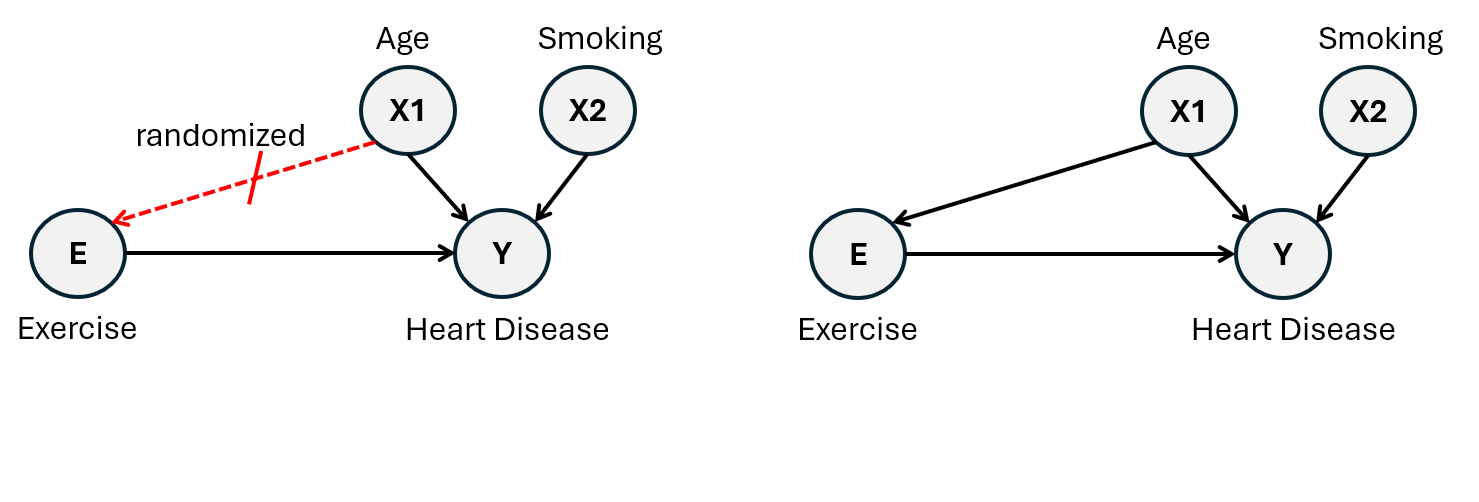
\includegraphics[width=\textwidth]{img/RCT_Observational.png}
% 
% 
% \end{frame}
% 
% % 
% % \begin{frame}{Causality: Example}
% %     \centering
% %     \vspace{0.2cm}
% % <<dag_smoking, echo=FALSE, fig.width=3, fig.height=3, out.width="40%">>=
% % theme_set(theme_dag())
% % 
% % # Set custom coordinates
% % coord_dag <- list(
% %   x = c(smoking = 0, age = 1, exercise = 2, heart = 2),
% %   y = c(smoking = 1.3, age = 1.5, exercise = 1.5, heart = 1.3)
% % )
% % 
% % smoking_ca_dag <- dagify(heart ~ smoking + age + exercise,
% %   smoking ~ age,
% %   labels = c(
% %     "heart" = "Heart Disease",
% %     "smoking" = "Smoking",
% %     "exercise" = "Exercise",
% %     "age" = "Age"
% %   ),
% %   #latent = "unhealthy",
% %   exposure = "smoking",
% %   outcome = "heart",
% %   coords = coord_dag
% % )
% % 
% % # plot with reduced size
% % ggdag(smoking_ca_dag, text = FALSE, use_labels = "label") + theme_void()
% % 
% % 
% % # Use label repel to avoid overlap with arrows
% % ggdag(smoking_ca_dag, text = TRUE) +
% % 	geom_dag_label(aes(label = label, fill = FALSE), 
% %                   label.size = 0.2,
% %                   size = 3.5, 
% %                   color = "black", 
% %                   segment.color = "black", 
% %                   segment.size = 0.2) +
% %   theme_void()
% % 
% % @
% % \end{frame}
% \begin{frame}{Structural Causal Model}
% 
% \textbf{SCM:} Describes the causal mechanism and probabilistic uncertainty
% 
% \vspace{0.2cm}
% 
% \begin{itemize}
%     \item $X_i$ = observed variable
%     \item $U_i$ = noise distribution
%     % \item $f$ = in our case: $X_2 = f(X_1, U) = h^{-1}(U_{\text{logis}} - \mathbf{x}^\top \boldsymbol{\beta})$
% \end{itemize}
% 
% \vfill
% 
% \centering
% 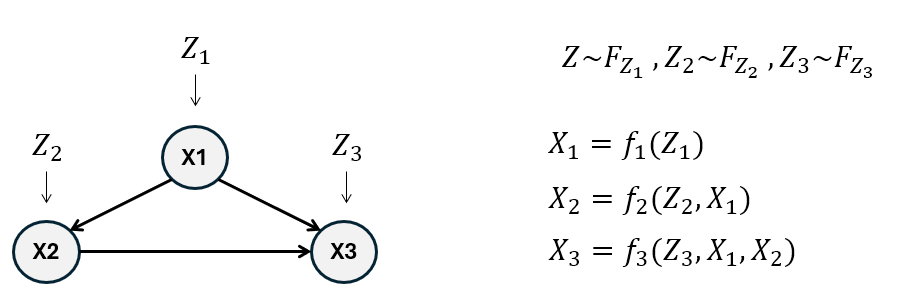
\includegraphics[width=1\textwidth]{img/SCM.png}
% 
% \end{frame}
% 
% 
% 
% 
% 
% 
% \begin{frame}{Estimating Functional Form}
% 
% % Statistical Methods
% \begin{columns}
% \begin{column}{0.75\textwidth}
% \textbf{Statistical methods:}
% \begin{itemize}
%     \item E.g. linear/logistic regression
%     \item Predefined form, risk of bias if misspecified
% \end{itemize}
% \end{column}
% \begin{column}{0.23\textwidth}
% 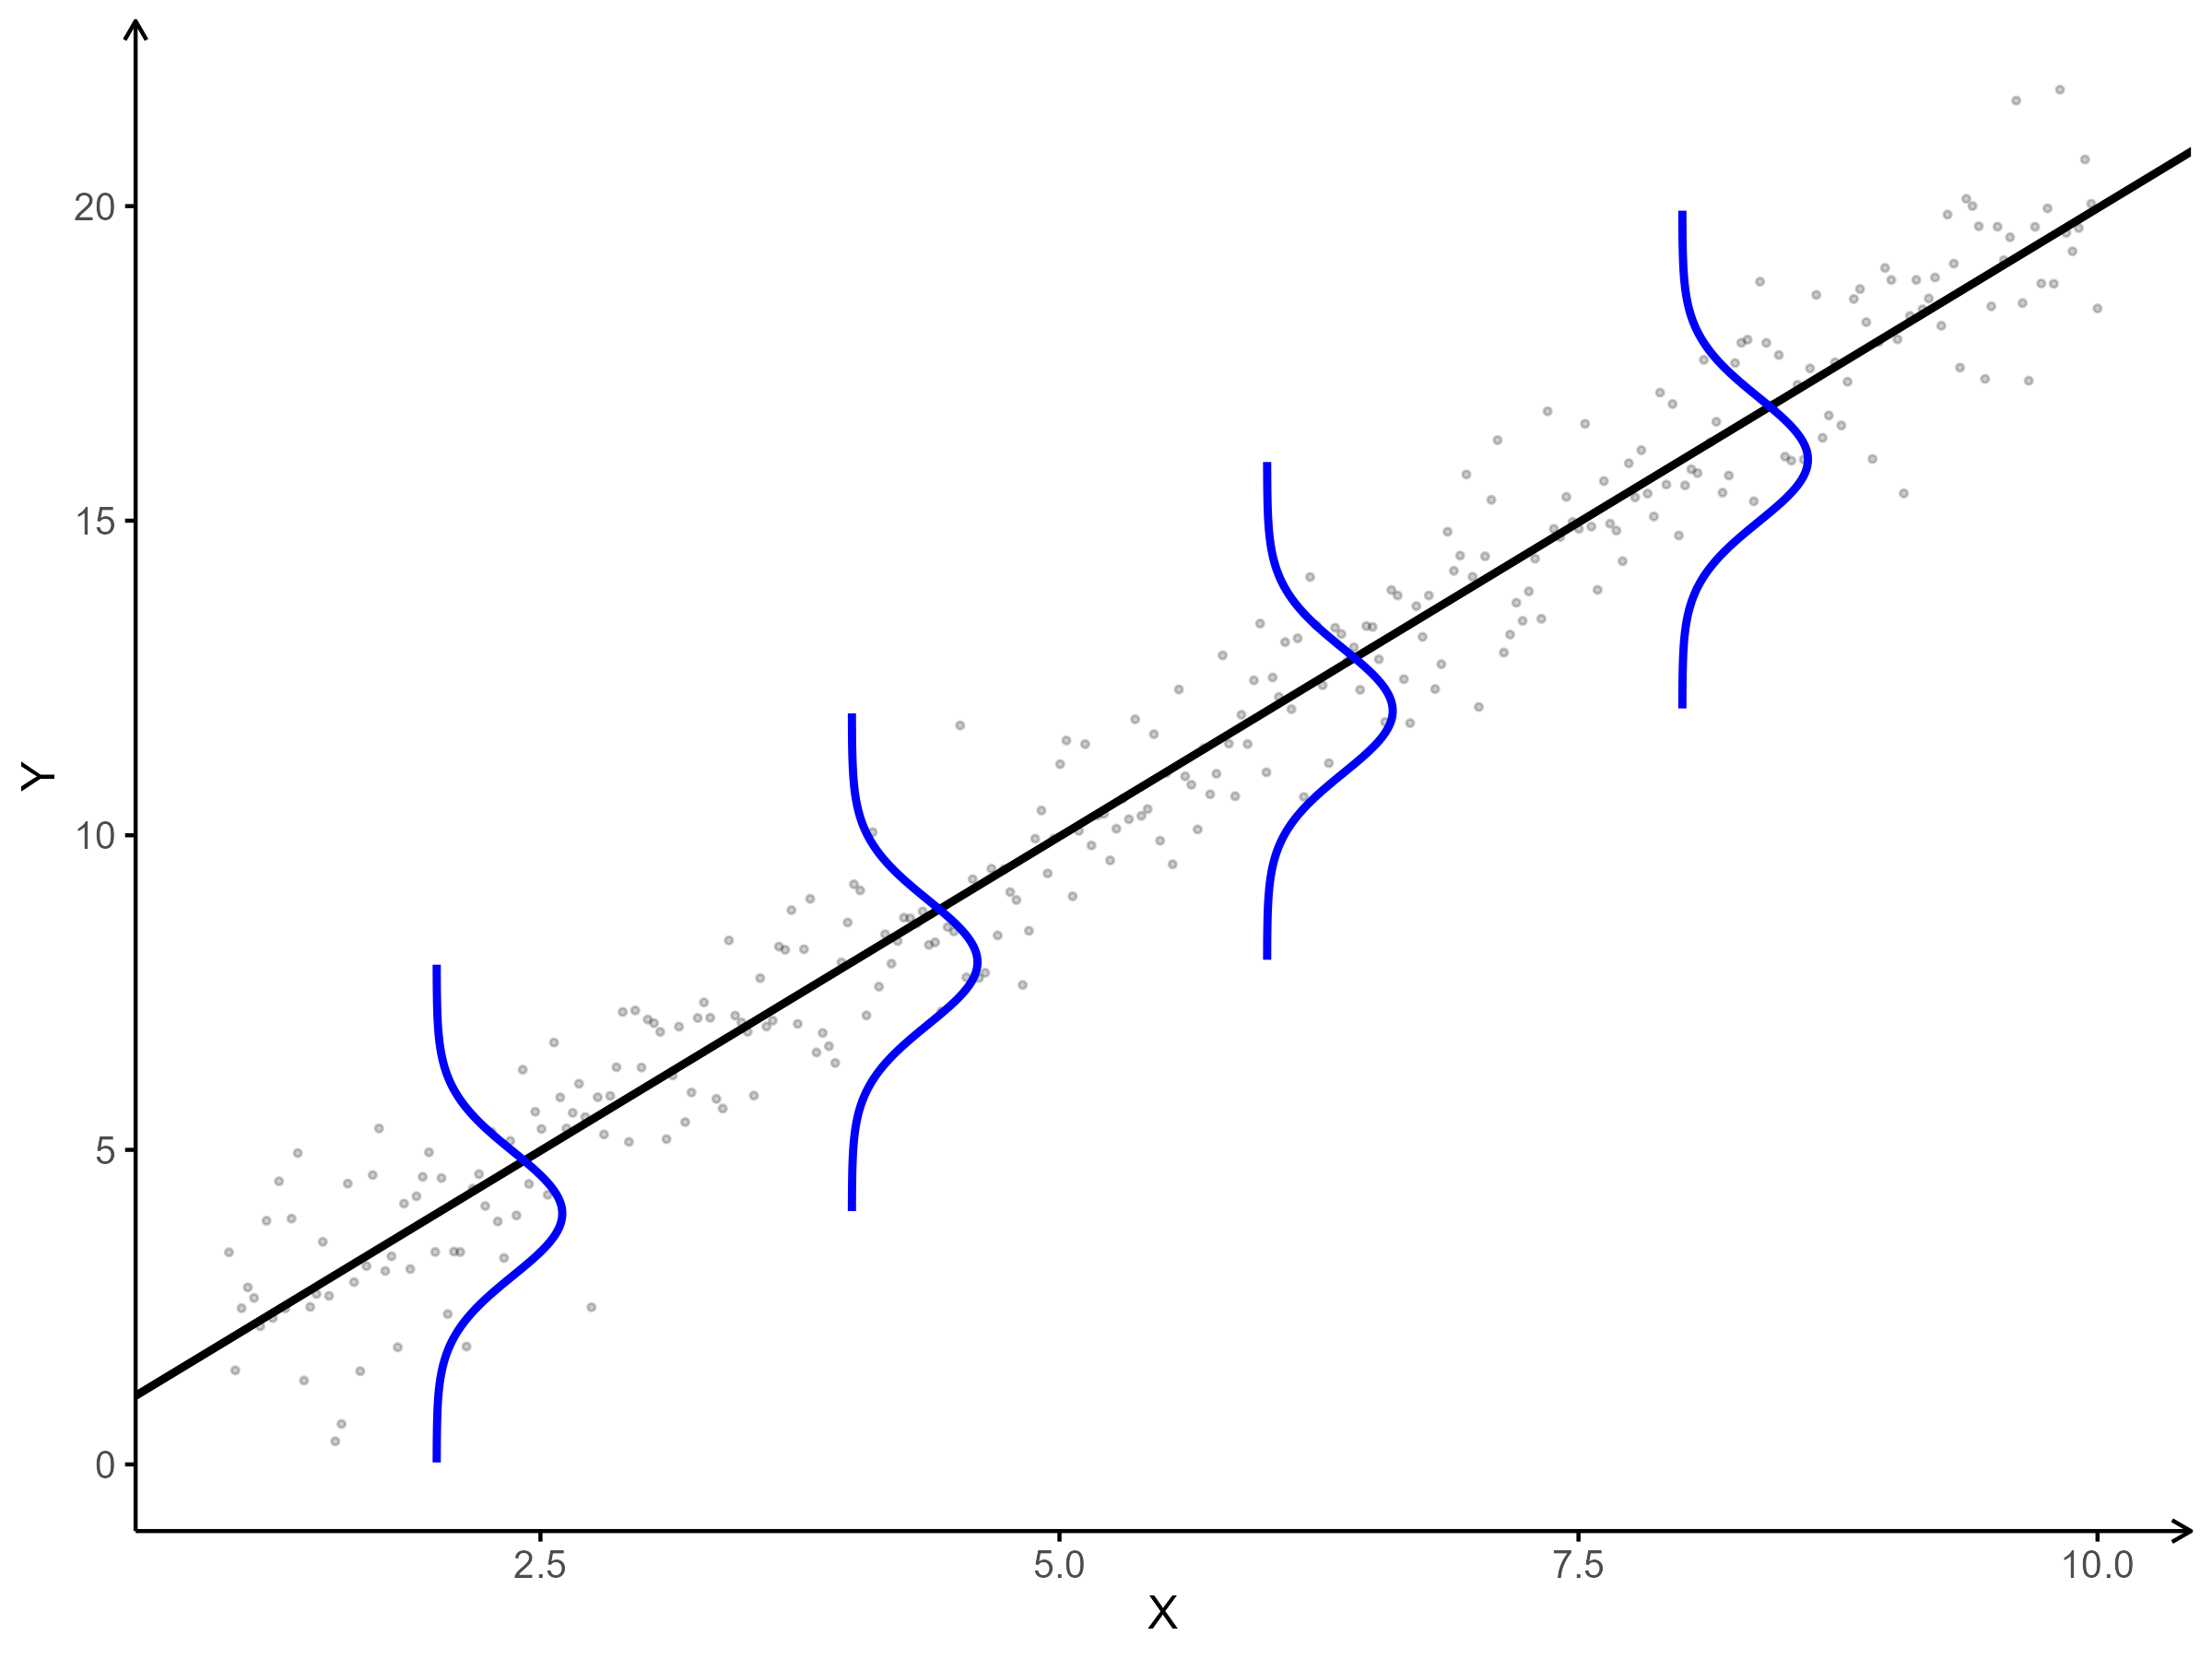
\includegraphics[width=\textwidth]{img/conditional_distributions.png}
% \end{column}
% \end{columns}
% 
% \vspace{0.3cm}
% 
% % Neural Networks
% \begin{columns}
% \begin{column}{0.75\textwidth}
% \textbf{Neural networks:}
% \begin{itemize}
%     \item E.g. feed-forward NNs, normalizing flows, VACAs
%     \item Flexible, but "black-box", data-type limitations
% \end{itemize}
% \end{column}
% \begin{column}{0.23\textwidth}
% 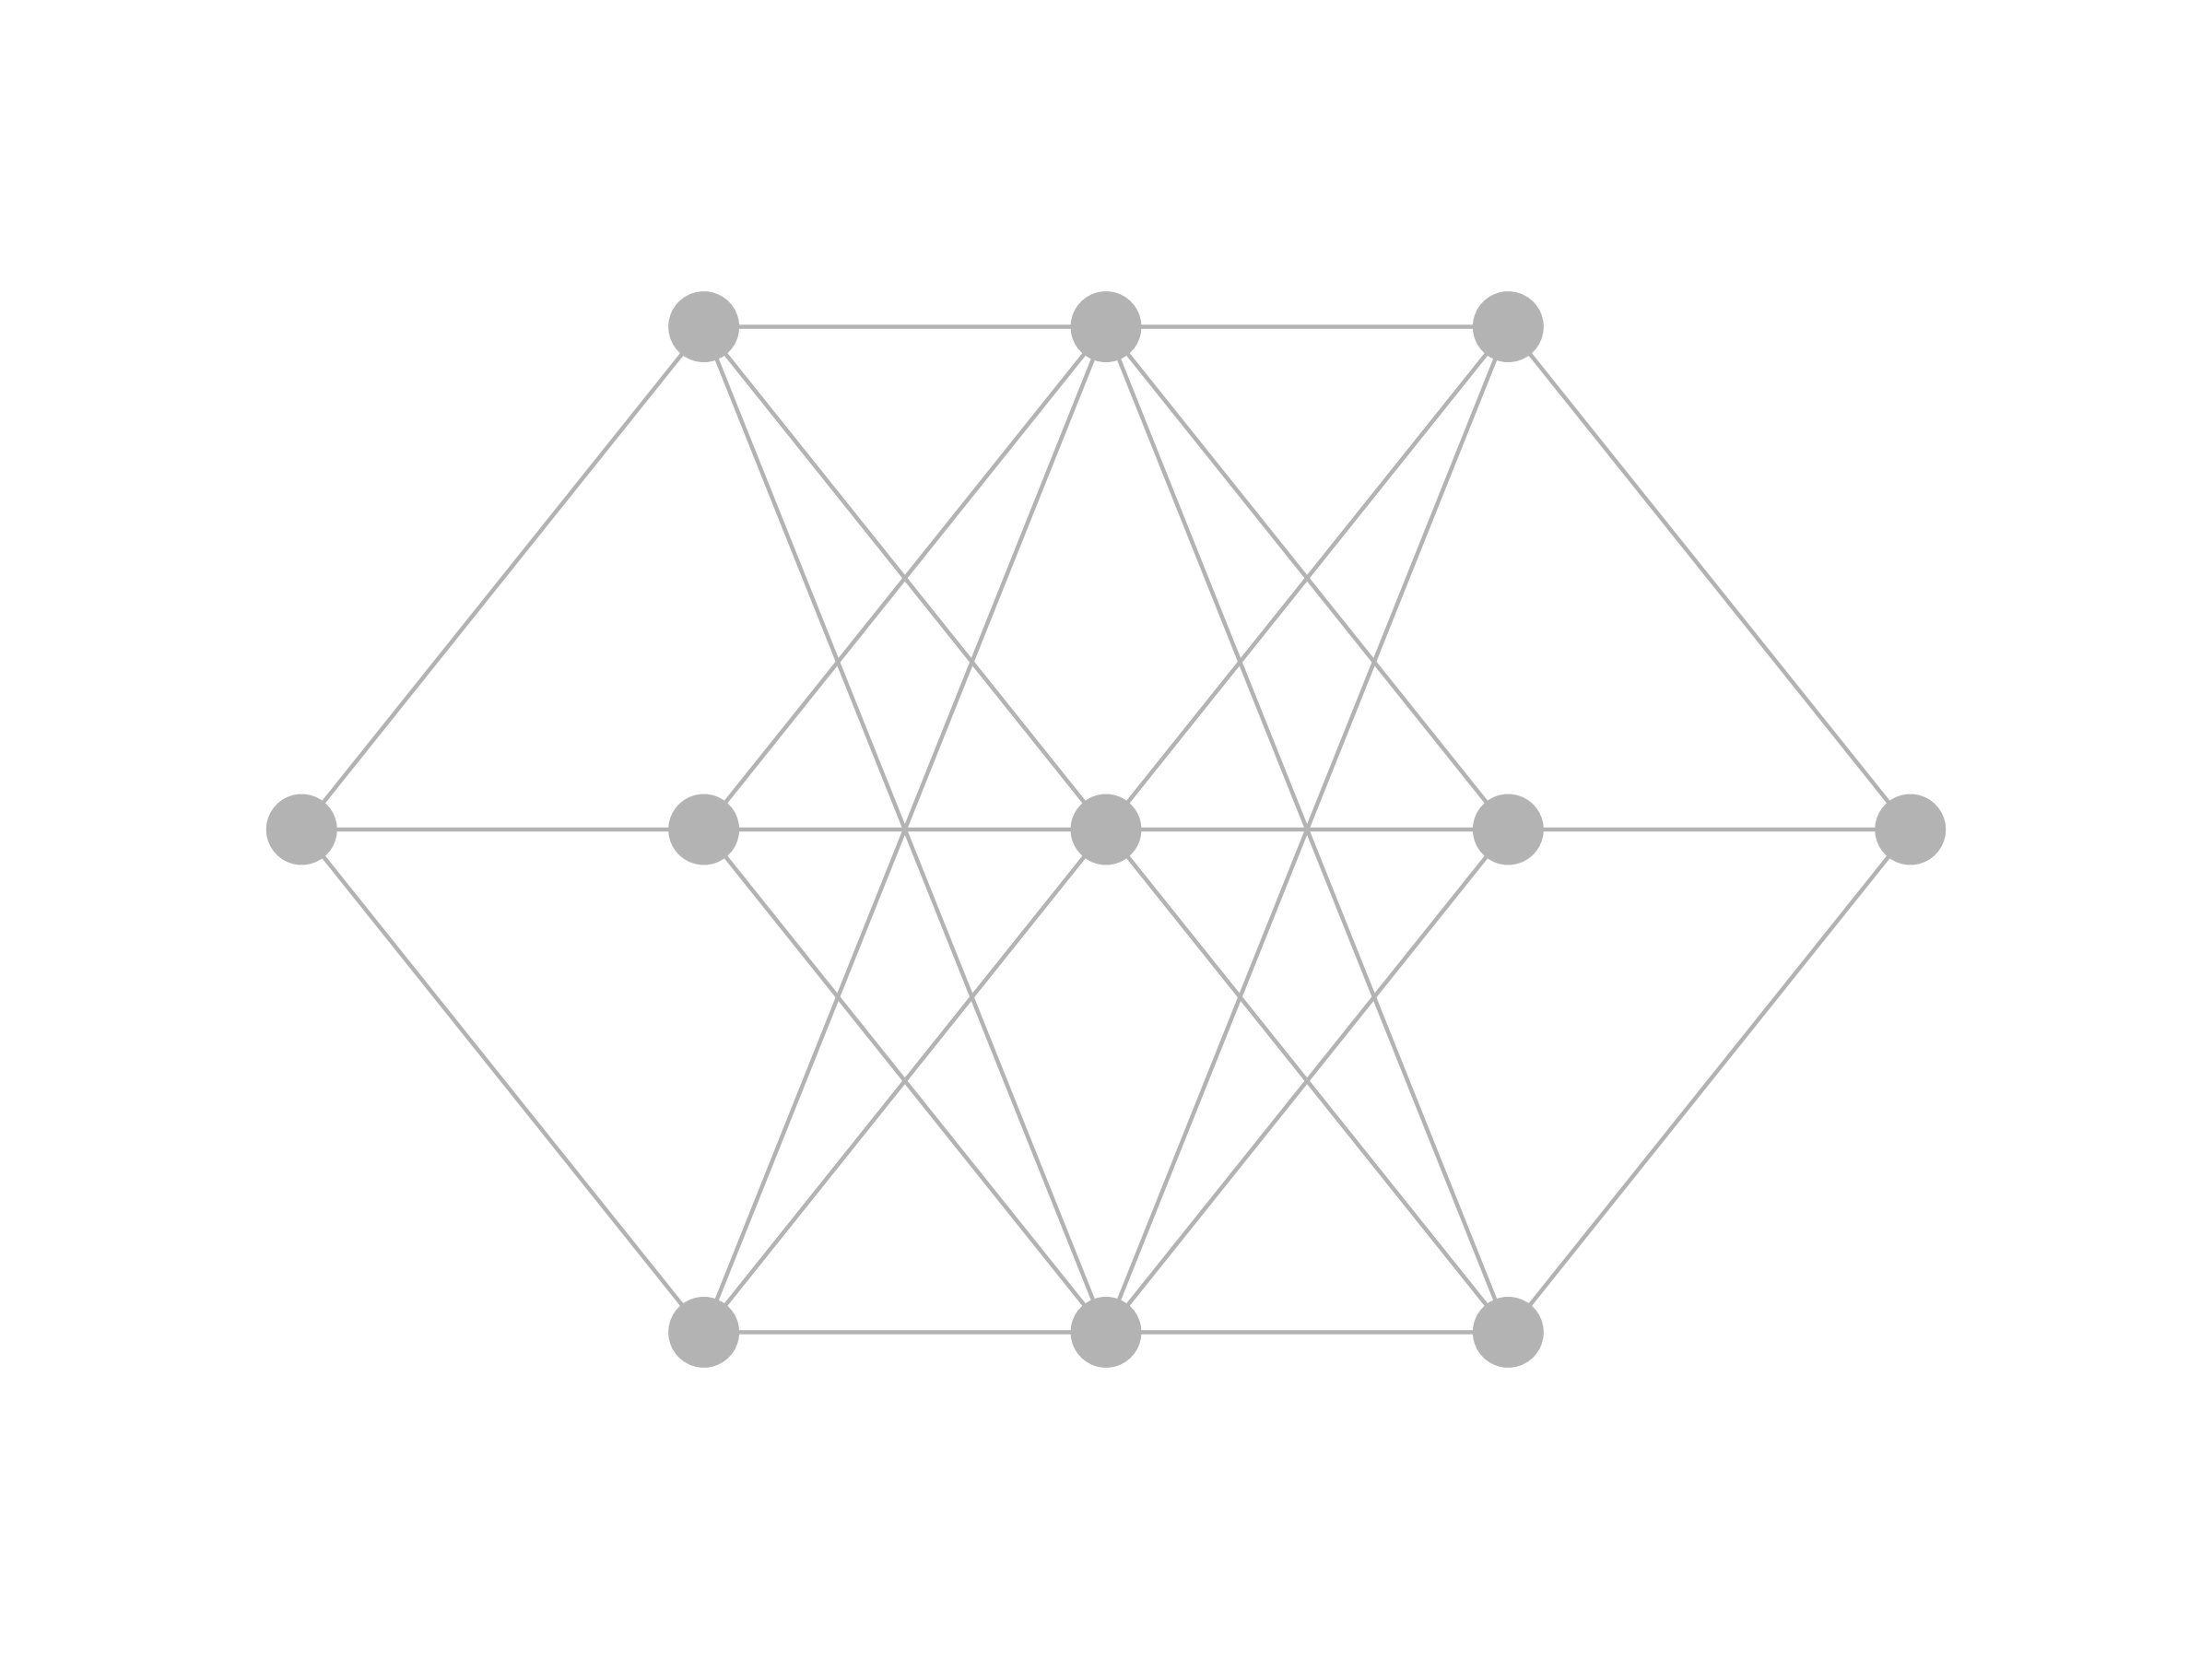
\includegraphics[width=\textwidth]{img/neural_network.png}
% \end{column}
% \end{columns}
% 
% \vspace{0.3cm}
% 
% % TRAM-DAGs
% \begin{columns}
% \begin{column}{0.75\textwidth}
% \textbf{TRAM-DAGs:}
% \begin{itemize}
%     \item Compromise: flexibility + interpretability
%     \item Mixed data types
% \end{itemize}
% \end{column}
% \begin{column}{0.23\textwidth}
% 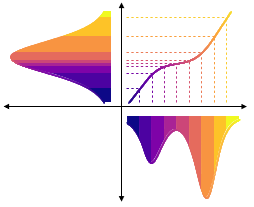
\includegraphics[width=\textwidth]{img/TRAM_Raw.png}
% \end{column}
% \end{columns}
% 
% \end{frame}
% 
% 
% 
% 
% 
% 
% 
% \begin{frame}{Pearl's Causality Ladder}
% 
% \begin{columns}
% 
% % Left side: Text (60%)
% \begin{column}{0.60\textwidth}
% 
% \textbf{Observational (seeing)} \\
% $P(Y=1 \mid E=1)$ \\
% {\footnotesize \textit{"Probability of heart disease given that the person exercises"}}
% 
% \vspace{0.4cm}
% 
% \textbf{Interventional (doing)} \\
% $P(Y=1 \mid \text{do}(E=1))$ \\
% {\footnotesize \textit{"Probability of heart disease if we made people start exercising"}} 
% 
% \vspace{0.4cm}
% 
% \textbf{Counterfactual (imagining)} \\
%  $P(Y_{(E=1)} = 1 \mid E=0, Y=1)$ \\
% {\footnotesize \textit{"Would someone who does not exercise and has heart disease still have it if they had exercised?"}}
% 
% \end{column}
% 
% % Right side: Image (40%)
% \begin{column}{0.40\textwidth}
% 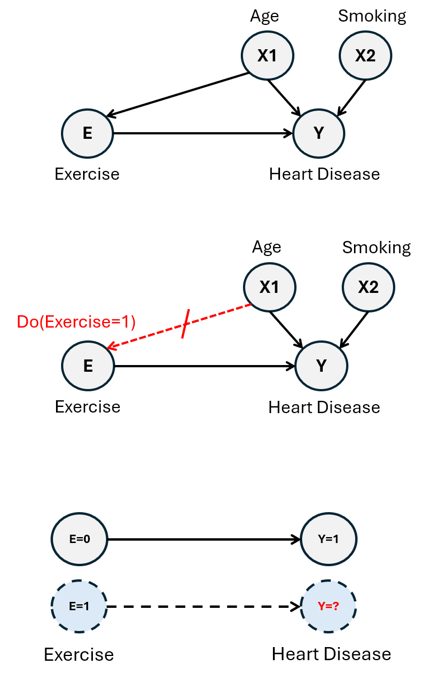
\includegraphics[width=1\linewidth]{img/Pearls_Ladder.png}
% \end{column}
% 
% \end{columns}
% 
% \end{frame}
% 
% 
% \begin{frame}{Individualized Treatment Effect (ITE)}
% 
% Difference in outcomes between two treatment options, for one specific individual with unique characteristics.
%     \[
%     \text{ITE}_\text{i} = \text{P}(\text{Y}_\text{i} = 1 \mid \text{T} = 1, \mathbf{X} = \mathbf{x_i}) - \text{P}(\text{Y}_\text{i} = 1 \mid \text{T} = 0, \mathbf{X} = \mathbf{x_i})
%     \]
%     
% \textbf{Difficulty:} \\
% \begin{itemize}
% 	% \item Personalized medicine
% 	\item We can only observe one facutal outcome - the other one is counterfactual
%     % \item \textbf{Average treatment effect:}
%     % \[
%     % \text{ATE} = \text{E}\left[\text{ITE}_i \right]
%     % \]
% \end{itemize}
% 
% 
% \begin{columns}
% 
% % Left side: Text
% \begin{column}{0.55\textwidth}
% 
% \textbf{Recent findings:} \\
% \begin{itemize}
%     \item \citet{chen2025} analyzed mainstream causal ML methods for ITE estimation on two large RCTs.
%     \item ITEs estimated
% from training data failed to generalize to the test data
%  \end{itemize}
% \end{column}
% 
% % Right side: Image
% \begin{column}{0.45\textwidth}
% 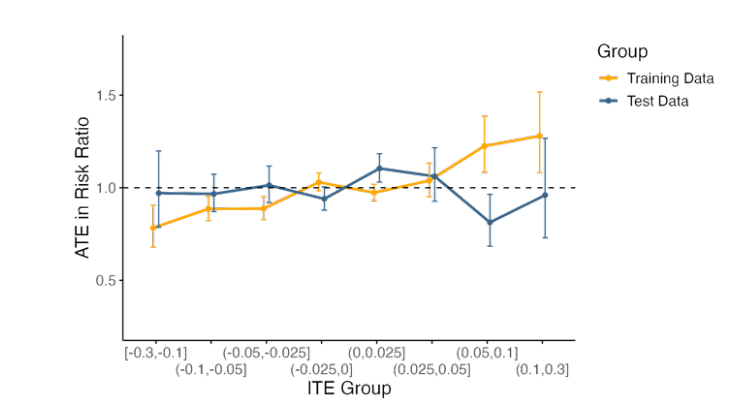
\includegraphics[width=\textwidth]{img/ATE_ITE.png}
% \end{column}
% \end{columns}
% 
% \end{frame}
% 
% 
% 
% 
% 
% \begin{frame}{Transformation Models}
% 
% Flexible distributional regression method \citep{hothorn2014}
% 
% \vspace{0.4cm}
% 
% \textbf{Continuous } $Y \in \mathbb{R}$: 
% \[
% F_{Y \mid \mathbf{X} = \mathbf{x}}(y) = F_Z(h(y) + \mathbf{x}^\top \boldsymbol{\beta})
% \]
% 
% \textbf{Discrete } $Y \in \{y_1, y_2, \ldots, y_K\}$: 
% \[
% P(Y \leq y_k \mid \mathbf{X} = \mathbf{x}) = F_Z(\vartheta_k + \mathbf{x}^\top \boldsymbol{\beta}), \quad k = 1, 2, \ldots, K - 1
% \]
% 
% \vspace{0.4cm}
% 
% \begin{itemize}
%     \item $F_Z$: CDF of the standard logistic distribution
%     \item $h$: Transformation function, monotonically increasing
%     \item $\mathbf{x}$: Predictors
% \end{itemize}
% 
% \end{frame}
% 
% 
% 
% 
% 
% 
% \begin{frame}{Transformation Models}
% 
% \begin{columns}
% 
% % Left column: Continuous Y
% \begin{column}{0.48\textwidth}
% \textbf{Continuous $Y$:}
% 
% {\small
% \vspace{0.2cm}
% Intercept: Bernstein polynomial
% \vspace{0.2cm}
% 
% \scalebox{0.85}{$
% h_I(y) = \frac{1}{M + 1} \sum_{k=0}^{M} \vartheta_k \, \text{B}_{k, M}(y)
% $}
% 
% \vspace{0.2cm}
% 
% \scalebox{0.85}{$
% h(y \mid \mathbf{x}) = h_I(y) - \mathbf{x}^\top \boldsymbol{\beta}
% $}
% }
% 
% \end{column}
% 
% % Right column: Discrete/Ordinal Y
% \begin{column}{0.48\textwidth}
% \textbf{Discrete/Ordinal $Y$:}
% 
% {\small
% 
% \vspace{0.2cm}
% Intercept: Cut-off value
% \vspace{0.2cm}
% 
% \scalebox{0.85}{$
% h_I(y_k) = \vartheta_k
% $}
% 
% \vspace{0.2cm}
% 
% \scalebox{0.85}{$
% h(y_k \mid \mathbf{x}) = h_I(y_k) - \mathbf{x}^\top \boldsymbol{\beta}
% $}
% }
% 
% \end{column}
% 
% \end{columns}
% 
% \vspace{0.3cm}
% \centering
% 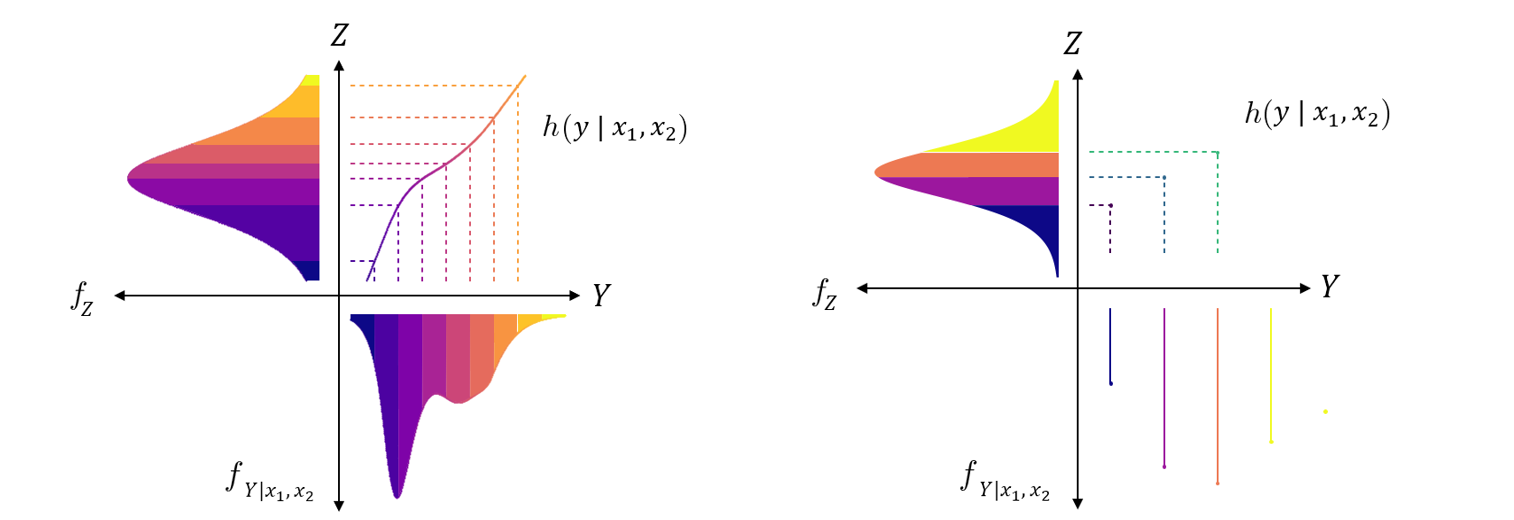
\includegraphics[width=0.9\textwidth]{img/TRAM_Cont_Ord.png}
% 
% \end{frame}
% 
% 
% 
% 
% 
% 
% 
% 
% \begin{frame}{Deep TRAMs}
%   \begin{itemize}
%     \item Extended to Deep TRAMs \citep{sick2020}
%     \item Flexible components
%     \item Minimize the NLL through NN optimization
%   \end{itemize}
% 
%   \vfill
%   \centering
%   \includegraphics[width=0.9\linewidth]{img/deep_TRAM.png}
% \end{frame}
% 
% 
% 
% 
% 
% \begin{frame}{TRAM-DAGs}
% 
%   \centering
%   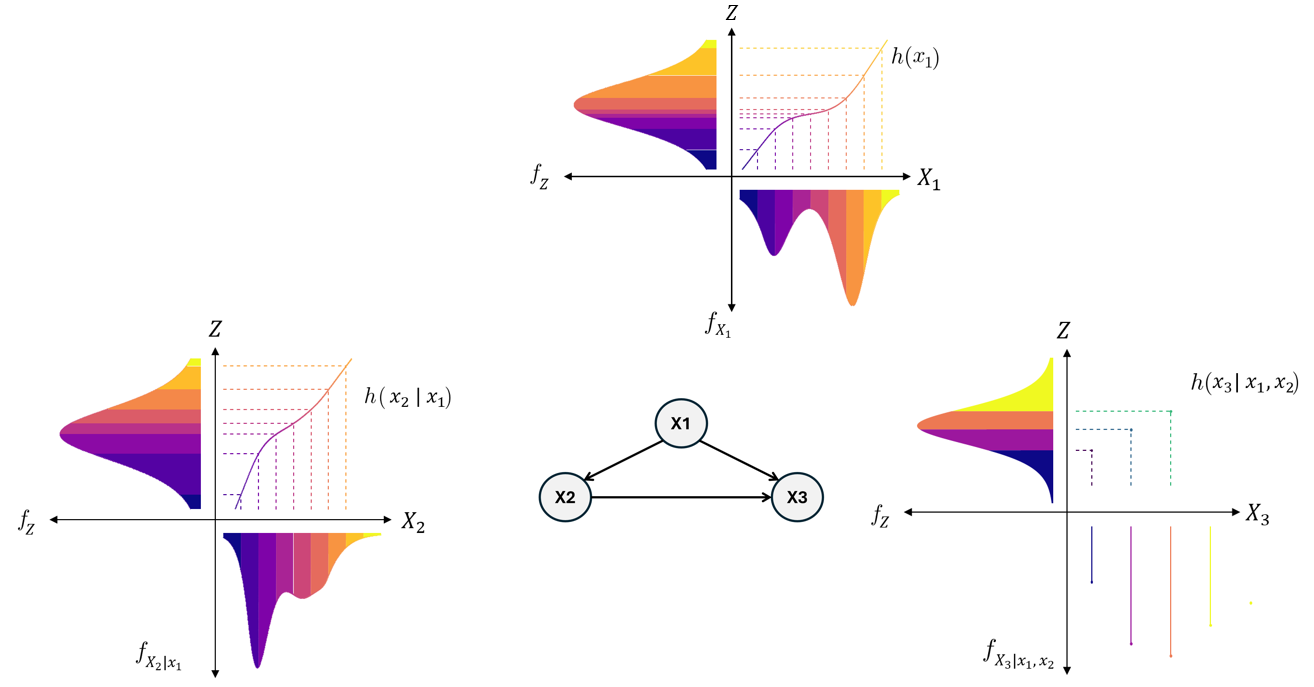
\includegraphics[width=1\linewidth]{img/TRAM_DAG.png}
% \end{frame}
% 
% 
% 
% \begin{frame}{Simulation Example}
%   \begin{itemize}
%     \item We have:
%     \begin{itemize}
%       \item Observational data (simulated)
%       \item Predefined DAG
%     \end{itemize}
%     \item We want:
%     \begin{itemize}
%       \item Estimate conditional CDF of each variable
%       \item Sample from conditional distributions for causal queries
%     \end{itemize}
%   \end{itemize}
% 
%   \vfill
%   \centering
%   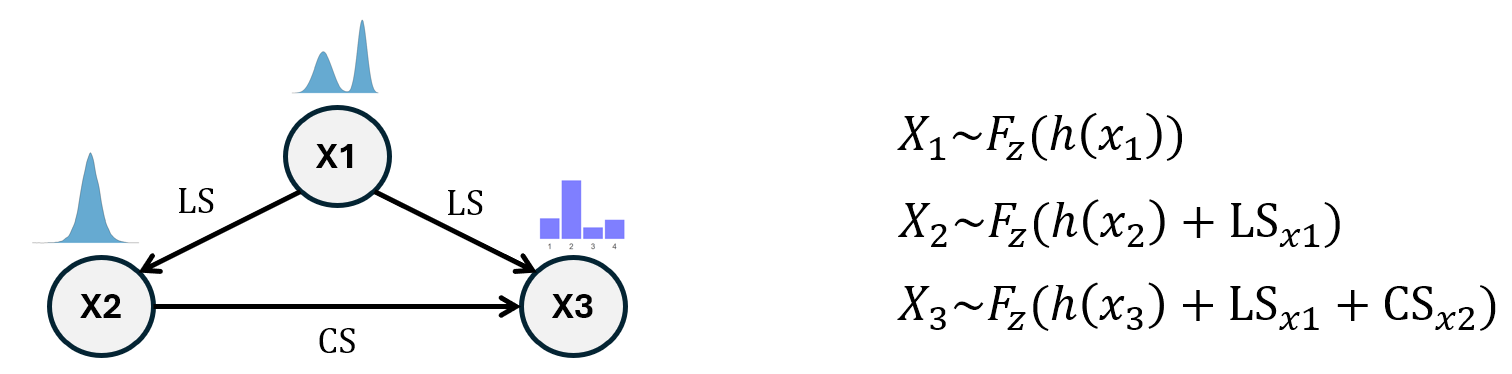
\includegraphics[width=0.7\linewidth]{img/Simulation_Example.png}
% \end{frame}
% 
% 
% 
% 
% \begin{frame}{Adjacency Matrix}
% 
% Model structure represented by a meta-adjacency matrix:
% 
% \begin{itemize}
%   \item \textbf{Rows}: source of effect
%   \item \textbf{Columns}: target of effect
% \end{itemize}
% 
% \vspace{0.4cm}
% 
% \begin{center}
% \begin{tikzpicture}[baseline={(current bounding box.center)}]
% 
%   % DAG image
%   \node (img) at (0, 0) {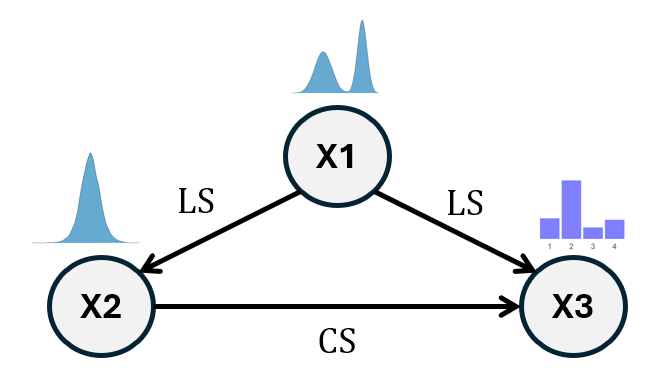
\includegraphics[width=0.28\textwidth]{img/DAG_MA.png}};
% 
%   % Matrix
%   \node (matrix) at (5, 0) {
%     $\mathbf{MA} =
%     \begin{bmatrix}
%       0 & \text{LS} & \text{LS} \\
%       0 & 0  & \text{CS} \\
%       0 & 0  & 0
%     \end{bmatrix}$
%   };
% 
%   % Arrow
%   \draw[->, thick] (img.east) -- (matrix.west);
% 
% \end{tikzpicture}
% \end{center}
% 
% \end{frame}
% 
% 
% 
% \begin{frame}{Data Generating Process (DGP)}
% 
% \begin{columns}
% 
% % Left column: Descriptions and formulas
% \begin{column}{0.72\textwidth}
% 
% \textbf{\(X_1\):} Continuous, bimodal. \textit{Source node} (independent).
% 
% \vspace{0.4cm}
% 
% \textbf{\(X_2\):} Continuous. Depends on \(X_1\) (\textcolor{red}{linear}):
% 
% \vspace{0.15cm}
% {\scriptsize
% \[
% \textcolor{red}{\beta_{12} = 2}, \quad h_I(X_2) = 5 X_2
% \]
% \[
% \boxed{
% h(X_2 \mid X_1) = h_I(X_2) + \textcolor{red}{\beta_{12}} X_1
% }
% \]
% }
% 
% \vspace{0.4cm}
% 
% \textbf{\(X_3\):} Ordinal. Depends on \(X_1\) (\textcolor{red}{linear}) and \(X_2\) (\textcolor{blue}{complex}):
% 
% \vspace{0.15cm}
% {\scriptsize
% \[
% \textcolor{red}{\beta_{13} = 0.2}, \quad \textcolor{blue}{f(X_2) = 0.5 \cdot \exp(X_2)}, \quad \vartheta_k \in \{-2,\, 0.42,\, 1.02\}
% \]
% \[
% \boxed{
% h(X_{3,k} \mid X_1, X_2) = \vartheta_k + \textcolor{red}{\beta_{13}} X_1 + \textcolor{blue}{f(X_2)}
% }
% \]
% }
% 
% \end{column}
% 
% % Right column: Plot
% \begin{column}{0.28\textwidth}
% 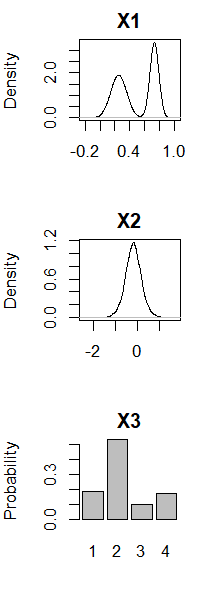
\includegraphics[width=0.8\linewidth]{img/DGP_Variables.png}
% \end{column}
% 
% \end{columns}
% 
% \end{frame}
% 
% 
% 
% 
% 
% % \textbf{Parameters:} 281 total (not all used)
% % \begin{itemize}
% %     \item Simple Intercepts (SI): \textbf{240} \\
% %     - only 43 needed (20 + 20 + 3)
% %     \item Linear Shifts (LS): \textbf{9} \\
% %     - 2 active
% %     \item Complex Shifts (CS): \textbf{32} \\
% %     - 24 active
% % \end{itemize}
% 
% % 
% % \begin{frame}{Construct Model: Modular Neural Network}
% % 
% % \begin{columns}
% % 
% % % Left side: Text
% % \begin{column}{0.65\textwidth}
% % 
% % \vspace{0.1cm}
% % 
% % \textbf{Inputs:} \\ Observations + adjacency matrix
% % 
% % \vspace{0.4cm}
% % 
% % \textbf{Outputs:}
% % \begin{itemize}
% %     \item Simple Intercepts (SI): \vartheta
% %     \item Linear Shifts (LS): $\beta_{12}X_1, \beta_{13}X_2$
% %     \item Complex Shift (CS):  $\beta(X_2)$
% % \end{itemize}
% % 
% % 
% % 
% % \vspace{0.4cm}
% % \textbf{Transformation Functions:} \\
% % \begin{align*}
% % h(X \mid pa(X)) = \text{SI} + \text{LS} + \text{CS} \\
% % & h(X_1) = h_I(X_1) \\
% % & h(X_2 \mid X_1) = h_I(X_2) + \textcolor{red}{\beta_{12} X_1} \\
% % & h(X_{3,k} \mid X_1, X_2) = \vartheta_k + \textcolor{red}{\beta_{13} X_1} + \textcolor{blue}{\beta(X_2)} 
% % % \quad \( h = \text{SI} + \text{LS} + \text{CS} \)
% % \end{align*}
% % \end{column}
% % 
% % % Right side: Image
% % \begin{column}{0.35\textwidth}
% % \begin{figure}
% %   \centering
% %   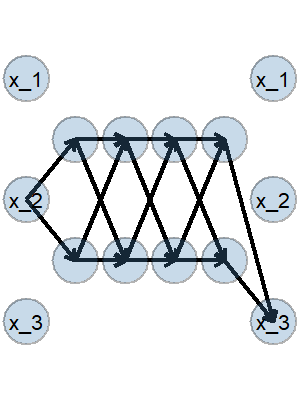
\includegraphics[width=0.65\linewidth]{img/CS.png}
% %   \caption{$\text{CS}_{X_2}$ on $X_3$}
% % \end{figure}
% % 
% % \end{column}
% % 
% % \end{columns}
% % 
% % \end{frame}
% % 
% 
% 
% \begin{frame}{Construct Model: Modular Neural Network}
% 
% \begin{columns}
% 
% % Left side: Text
% \begin{column}{0.65\textwidth}
% 
% \vspace{0.1cm}
% 
% \textbf{Inputs:} \\ Observations + adjacency matrix
% 
% \vspace{0.4cm}
% 
% \textbf{Outputs:}
% \begin{itemize}
%     \item Simple Intercepts (SI): $\textcolor{violet}{\vartheta}$
%     \item Linear Shifts (LS): $\textcolor{red}{\beta_{12}X_1}, \textcolor{red}{\beta_{13}X_2}$
%     \item Complex Shift (CS):  $\textcolor{blue}{\beta(X_2)}$
% \end{itemize}
% 
% \vspace{0.4cm}
% \textbf{Transformation Functions:}
% \begin{align*}
% & \boxed{h(X_i \mid pa(X_i)) = \text{SI} + \text{LS} + \text{CS}} \\
% & h(X_1) = \textcolor{violet}{h_I(X_1)} \\
% & h(X_2 \mid X_1) = \textcolor{violet}{h_I(X_2)} + \textcolor{red}{\beta_{12} X_1} \\
% & h(X_{3,k} \mid X_1, X_2) = \textcolor{violet}{\vartheta_k} + \textcolor{red}{\beta_{13} X_1} + \textcolor{blue}{\beta(X_2)} 
% \end{align*}
% 
% \end{column}
% 
% % Right side: Image
% \begin{column}{0.35\textwidth}
% \begin{figure}
%   \centering
%   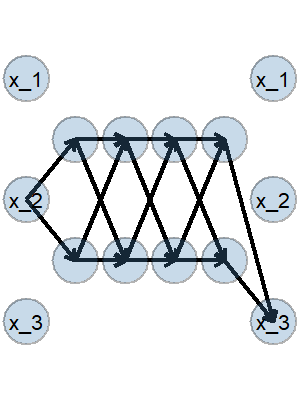
\includegraphics[width=0.65\linewidth]{img/CS.png}
%   \caption{$\text{CS}_{X_2}$ on $X_3$}
% \end{figure}
% \end{column}
% 
% \end{columns}
% 
% \end{frame}
% 
% 
% % 
% % \begin{frame}{The Setting}
% % 
% % \begin{columns}
% % 
% % % Left column: What we have
% % \begin{column}{0.48\textwidth}
% % \textbf{What we have:}
% % \begin{itemize}
% %     \item Data
% %     \item DAG (expert knowledge or structure discovery)
% %     \item No hidden confounding
% %     \item Adjacency matrix
% % \end{itemize}
% % \end{column}
% % 
% % % Right column: What we want
% % \begin{column}{0.48\textwidth}
% % \textbf{What we want:}
% % \begin{itemize}
% %     \item Model each variable as a function of its parents
% %     \item Use transformation models: $F_Z(h(y \mid x))$
% %     \item Perform causal inference:
% %     \begin{itemize}
% %         \item Sample from observational distribution
% %         \item Sample from interventional distribution
% %         \item Answer counterfactual queries
% %     \end{itemize}
% % \end{itemize}
% % \end{column}
% % 
% % \end{columns}
% % 
% % \end{frame}
% 
% 
% 
% % Simulation experiment from the file:
% % experiment_5_ordinal_outcome.R
% 
% % 
% % \begin{frame}{Loss: Negative Log-Likelihood (NLL)}
% % 
% % % Emphasized core components
% % \textbf{CDF, density and NLL of the TRAM (for continuous outcome):}
% % \[
% % F_{Y \mid \mathbf{X} = \mathbf{x}}(y) = F_Z (h(s(y) \mid \mathbf{x}))
% % \]
% % 
% % \[
% % f_{Y \mid \mathbf{X} = \mathbf{x}}(y) = f_Z (h(s(y) \mid \mathbf{x})\right) \cdot h'\left(s(y) \mid \mathbf{x}\right) \cdot s'(y)
% % \]
% % 
% % \[
% % \begin{aligned}
% % \text{NLL} = - \log f_{Y \mid \mathbf{X} = \mathbf{x}}(y)
% % &= -h(s(y) \mid \mathbf{x}) - 2 \log\left(1 + \exp\left(-h(s(y) \mid \mathbf{x})\right)\right) \\
% % &\quad + \log h'(s(y) \mid \mathbf{x}) - \log(\max(y) - \min(y))
% % \end{aligned}
% % \]
% % 
% % \vspace{0.4cm}
% % 
% % % Supporting details in smaller columns
% % \begin{columns}
% % \begin{column}{0.5\textwidth}
% % {\scriptsize
% % \textbf{Standard Logistic Density:}
% % \[
% % f_Z(z) = \frac{e^{z}}{(1 + e^{z})^2}, \quad z \in \mathbb{R}
% % \]
% % }
% % \end{column}
% % 
% % \begin{column}{0.5\textwidth}
% % {\scriptsize
% % \textbf{Scaled $y$ (Bernstein Polynomial on $[0,1]$):}
% % \[
% % s(y) = \frac{y - \min(y)}{\max(y) - \min(y)}
% % \]
% % }
% % \end{column}
% % \end{columns}
% % 
% % \end{frame}
% 
% 
% 
% 
% \begin{frame}{Loss: Negative Log-Likelihood (NLL)}
% 
% % Emphasized core components
% \textbf{CDF, density and NLL of the TRAM (for continuous outcome):}
% \[
% F_{Y \mid \mathbf{X} = \mathbf{x}}(y) = F_Z(h(s(y) \mid \mathbf{x}))
% \]
% 
% \[
% f_{Y \mid \mathbf{X} = \mathbf{x}}(y) = f_Z(h(s(y) \mid \mathbf{x})) \cdot h'(s(y) \mid \mathbf{x}) \cdot s'(y)
% \]
% 
% 
% \[
% \text{NLL} = - \log (f_{Y \mid \mathbf{X} = \mathbf{x}}(y))
% \]
% 
% %  full NLL
% % \[
% % \begin{aligned}
% % \text{NLL} = - \log f_{Y \mid \mathbf{X} = \mathbf{x}}(y)
% % &= -h(s(y) \mid \mathbf{x}) - 2 \log(1 + \exp(-h(s(y) \mid \mathbf{x}))) \\
% % &\quad + \log h'(s(y) \mid \mathbf{x}) - \log(\max(y) - \min(y))
% % \end{aligned}
% % \]
% 
% \vspace{0.4cm}
% 
% % Supporting details in smaller columns
% \begin{columns}
% \begin{column}{0.5\textwidth}
% {\scriptsize
% \textbf{Standard logistic density:}
% \[
% f_Z(z) = \frac{e^{z}}{(1 + e^{z})^2}, \quad z \in \mathbb{R}
% \]
% }
% \end{column}
% 
% \begin{column}{0.5\textwidth}
% {\scriptsize
% \textbf{Scaled $y$ (Bernstein polynomial bounded $[0,1]$):}
% \[
% s(y) = \frac{y - \min(y)}{\max(y) - \min(y)}
% \]
% }
% \end{column}
% \end{columns}
% 
% \end{frame}
% 
% 
% 
% 
% \begin{frame}{Model Fitting}
%   \begin{columns}
%     \begin{column}{0.5\linewidth}
%       \begin{itemize}
%         \item Samples: 20'000 training / 5'000 validation
%         \item Learning rate: 0.005
%         \item Epochs: 400
%       \end{itemize}
%     \end{column}
%     \begin{column}{0.5\linewidth}
%       \centering
%       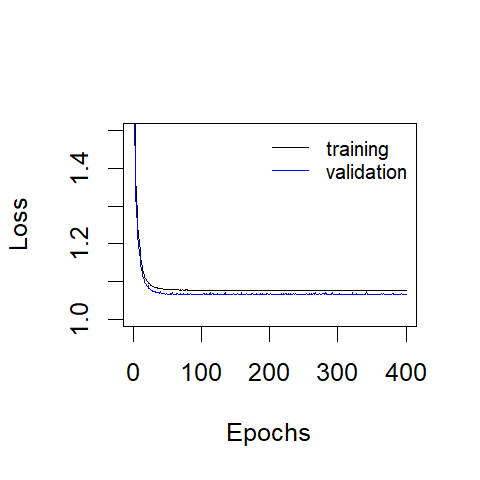
\includegraphics[width=\linewidth]{img/Loss_Example.png}
%     \end{column}
%   \end{columns}
% \end{frame}
% 
% 
% 
% 
% 
% 
% \begin{frame}{Interpretable Coefficients}
% 
% \begin{columns}
% 
% % Left column: Smaller formulas
% \begin{column}{0.42\textwidth}
% 
% \textbf{Linear Shift Coefficients:}
% 
% \vspace{0.2cm}
% 
% {\scriptsize
% \[
% F(x_2 \mid x_1) = F_Z\left(h(x_2) - x_1 \textcolor{red}{\beta_{12}}\right)
% \]
% 
% 
% \[
% F(x_3 \mid x_1, x_2) = F_Z\left(h(x_3) - x_1 \textcolor{red}{\beta_{13}} - CS_{x_2}\right)
% \]
% }
% 
% \end{column}
% 
% % Right column: Bigger plot
% \begin{column}{0.58\textwidth}
% 
% 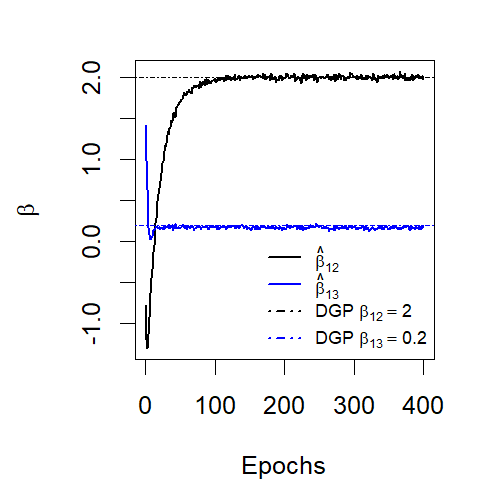
\includegraphics[width=\linewidth]{img/Betas.png}
% 
% \end{column}
% 
% \end{columns}
% 
% \end{frame}
% 
% 
% 
% 
% 
% 
% \begin{frame}{Interpretable Coefficients}
% \small
% \[
% F_{X_2 \mid X_1}(x_2) = \operatorname{expit}( h(x_2) + \beta_{12} x_1)
% \]
% 
% \vspace{0.3cm}
% 
% \[
% \log\left( \frac{F_{X_2 \mid X_1}(x_2)}{1 - F_{X_2 \mid x_1}(x_2)} \right)
% = \text{expit}^{-1}( \text{expit}(h(x_2) + \beta_{12} x_1 ))
% = h(x_2) + \beta_{12} x_1
% \]
% 
% \vspace{0.3cm}
% 
% \[
% \begin{aligned}
% \text{OR}_{x_1 \to x_1 + 1}
% &= \frac{\text{odds}(X_2 \le x_2 \mid X_1 = x_1 + 1)}{\text{odds}(X_2 \le x_2 \mid X_1 = x_1)} = \frac{\exp(h(x_2) + \beta_{12}(x_1 + 1))}{\exp(h(x_2) + \beta_{12} x_1)} = \exp(\beta_{12})
% \end{aligned}
% \]
% 
% \vspace{0.4cm}
% 
% \textbf{Interpretation:} \\
% \(\exp(\beta_{12})\) is the \textbf{multiplicative change in odds} for \(X_2 \le x_2\) when increasing \(\mathbf{X}_1\) by 1 unit, \emph{holding all else constant}.
% 
% \end{frame}
% 
% 
% 
% 
% 
% 
% 
% \begin{frame}{Linear and Complex Shifts}
% 
% 
% 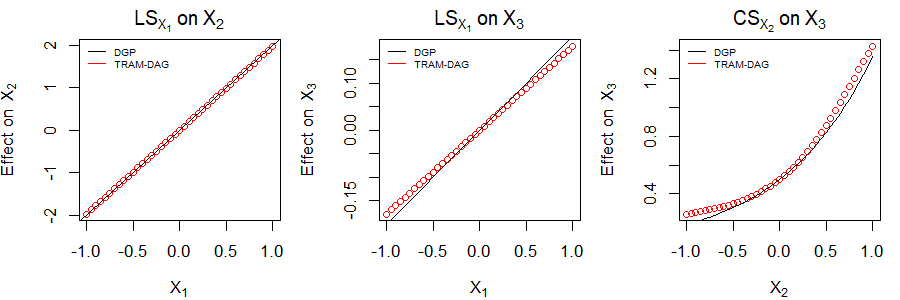
\includegraphics[width=\linewidth]{img/LS_CS.png}
% 
% 
% \end{frame}
% 
% 
% 
% 
% 
% 
% \begin{frame}{Intercepts}
% 
% 
% 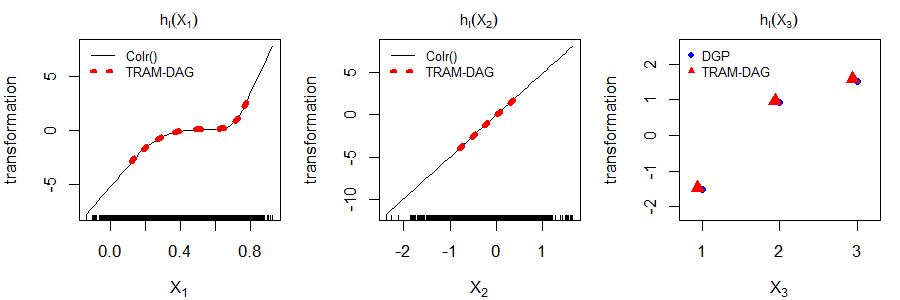
\includegraphics[width=\linewidth]{img/baseline_trafo.png}
% 
% 
% \end{frame}
% 
% 
% 
% \begin{frame}{What is Possible with a Fitted TRAM-DAG?}
% 
% Once the model is fitted, it can be used:
% 
% \begin{itemize}
% \item as genearative sampling model to sample observational and interventional distributions
% \item or to determine counterfactual outcomes in the continuous case.
% \end{itemize}
% 
% 
% Even if the model is fitted on observational data, we can make interventional and counterfactual statements, given the DAG is correct and no unobserved confounding.
% 
% 
% \end{frame}
% 
% 
% 
% \begin{frame}{Sampling from the Fitted TRAM-DAG (observational)}
% 
% \begin{columns}
% 
% % Left column: Sampling explanation
% \begin{column}{0.65\textwidth}
% 
% \textbf{Nodes $X_i , i \in \{1,\, 2,\, 3\}$:}
% 
% \vspace{0.2cm}
% 
% \begin{itemize}
%     \item Sample latent value: 
%     \[
%     z_i \sim F_{Z_i} \quad \text{(e.g., \texttt{rlogis()} in R)}
%     \]
% 
%     \item Determine \(x_i\) such that:
% 
%     \begin{itemize}
%         \item \textbf{If \(X_i\) is continuous:}
%         \[
%         x_i = h^{-1}(z_i \mid \text{pa}(x_i))
%         \]
%         
%         \item \textbf{If \(X_i\) is ordinal:}
%         find the smallest category $x_i$ such that
%         \[
%         x_i = \min \left\{ x : z_i \le h(x \mid \text{pa}(x_i)) \right\}
%         \]
%     \end{itemize}
% \end{itemize}
% 
% \end{column}
% 
% % Right column: Illustration
% \begin{column}{0.3\textwidth}
% 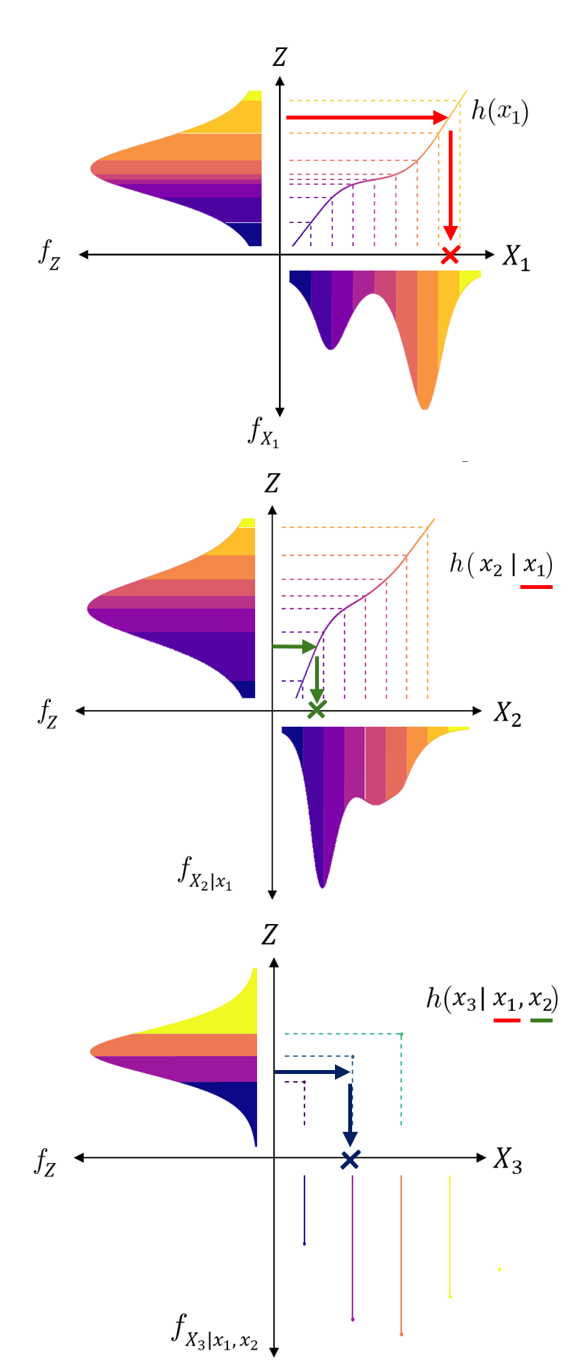
\includegraphics[width=0.9\linewidth]{img/Sampling.png}
% \end{column}
% 
% \end{columns}
% 
% \end{frame}
% 
% 
% 
% 
% \begin{frame}{Sampling from the Fitted TRAM-DAG (interventional)}
% 
% \textbf{Interventional sampling:} \\
% 
% \begin{itemize}
%     \item Do-intervention: \( \textcolor{red}{\text{do}(x_2 = \alpha})\)
%     \item Sample from the interventional-distribution:
% \end{itemize}
% \[
% x_3 = \min \left\{ x : z_3 \le h(x \mid x_1, \textcolor{red}{x_2 = \alpha}) \right\}
% \]
% 
% \centering
% 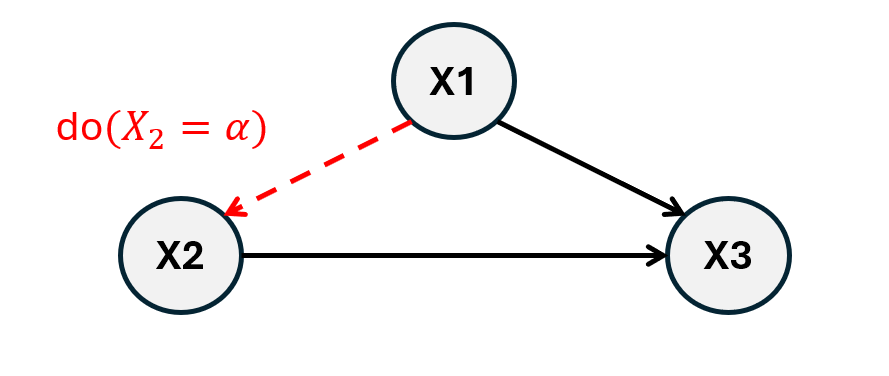
\includegraphics[width=0.5\linewidth]{img/interventional.png}
% 
% 
% \end{frame}
% 
% 
% \begin{frame}{Sampling Distributions}
% 
% 
% \begin{columns}
% 
% \begin{column}{0.75\linewidth}
%     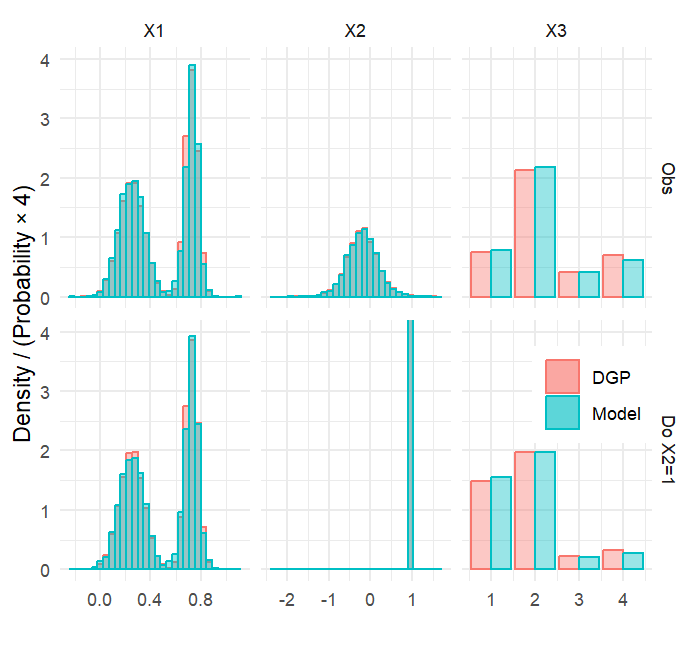
\includegraphics[width=1\linewidth]{img/Sampling_Distributions.png}
%   \end{column}
%   
%   
%   \begin{column}{0.25\linewidth}
%     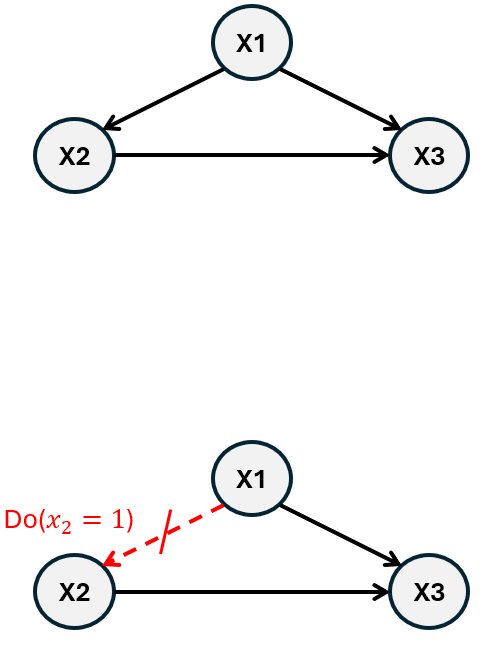
\includegraphics[width=1\linewidth]{img/Do_sampling.png}
%   \end{column}
%   
% \end{columns}
% 
% 
% 
% \end{frame}
% 
% 
% 
% 
% %  new slide for the image Prob_Estimates.png
% 
% \begin{frame}{Observational and Interventional Queries}
% 
% 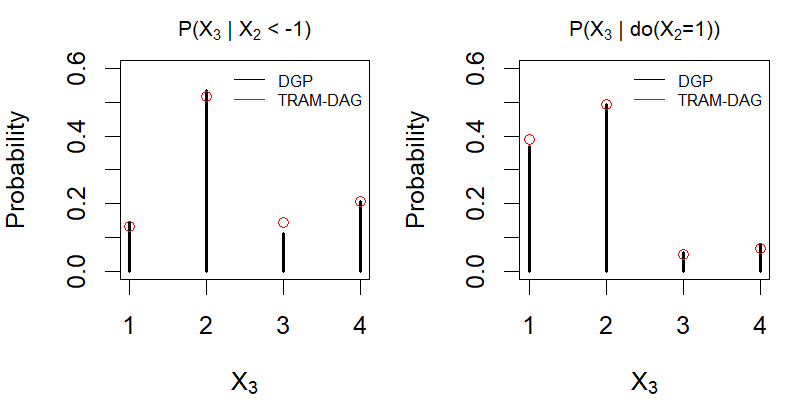
\includegraphics[width=1\linewidth]{img/Prob_Estimates.png}
% 
% \end{frame}
% 
% 
% 
% 
% \begin{frame}{Example: ITE Estimation}
% 
% 
% \centering
% 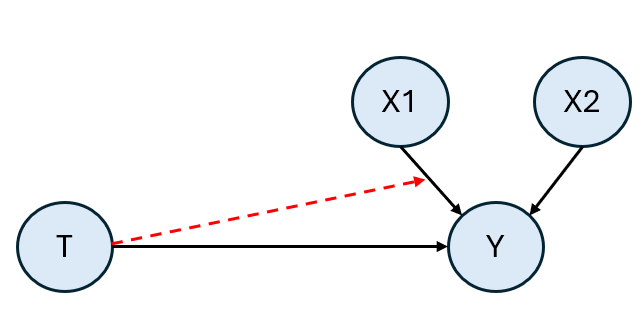
\includegraphics[width=0.3\linewidth]{img/ITE_DAG.png}
% 
% % \begin{columns}
% % 
% % % Left column: formulas + two images
% % \begin{column}{0.75\textwidth}
% \scriptsize
% 
% \vspace{0.2cm}
% \textbf{DGP:} \quad
% $\text{logit}(P(Y=1 \mid T, X_1, X_2)) = \beta_0 + X_1 \beta_1 + X_2 \beta_2 + T \beta_3 + \textcolor{red}{T X_1\beta_4}$
% 
% \vspace{0.2cm}
% 
% \textbf{TRAM-DAG:} \quad
% $h(Y_k \mid T, X_1, X_2) = \vartheta_k + \textcolor{red}{\text{CS}(T, X_1)} + \text{LS}(X_2)$
% 
% % \end{column}
% 
% % Right column: small DAG image
% % \begin{column}{0.25\textwidth}
% % \vspace{-0.2cm}
% % \centering
% % 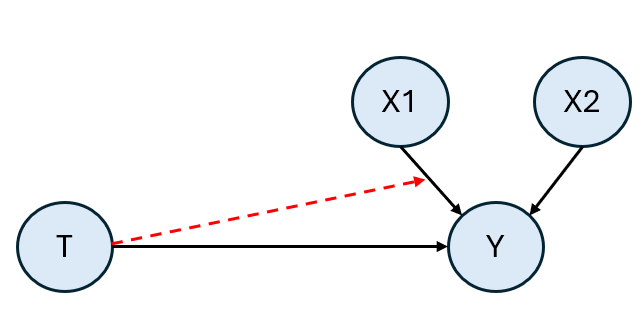
\includegraphics[width=1\linewidth]{img/ITE_DAG.png}
% % \end{column}
% 
% % \end{columns}
% 
% \vspace{-0.1cm}
% 
% \begin{columns}
% 
% % Small left image
% \begin{column}{0.48\textwidth}
% \begin{figure}
%   \centering
%   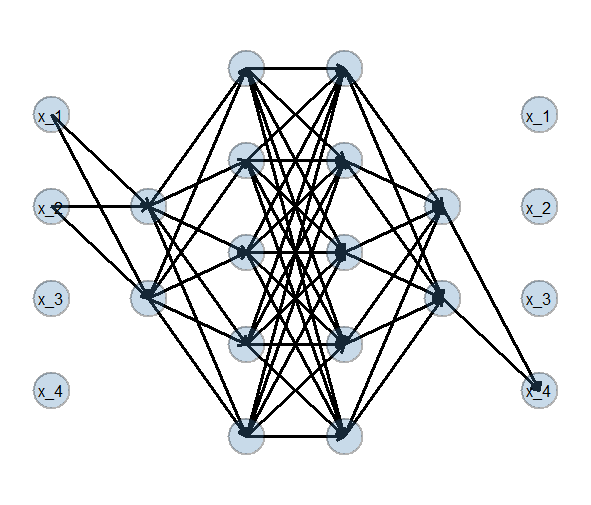
\includegraphics[width=0.7\linewidth]{img/NN_CS_T_X1.png}
%   \caption{$\text{CS}_{(T, X_1)}$ on $Y$}
% \end{figure}
% \end{column}
% 
% % Wide right image
% \begin{column}{0.48\textwidth}
% \centering
% 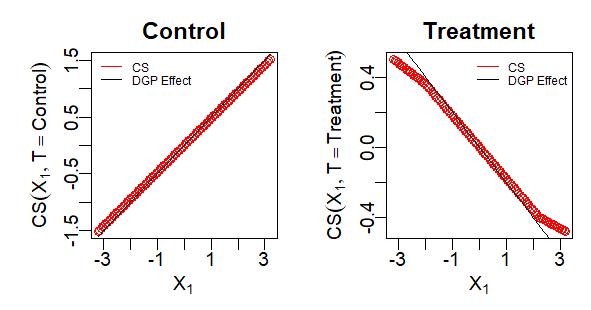
\includegraphics[width=\linewidth]{img/CS_T_X1.png}
% \end{column}
% 
% \end{columns}
% 
% 
% 
% \end{frame}
% 
% 
% \begin{frame}{Example: ITE Estimation}
% 
% \begin{columns}
% % Left column: text
% \begin{column}{0.5\textwidth}
% \textbf{ITE\textsubscript{i} estimation from fitted model:}
% 
% \begin{itemize}
% 	\item \(\text{P}(\text{Y}_\text{i} = 1 \mid \textcolor{red}{\text{do(T = 1)}}, \mathbf{x_i})\)
% 	\item \(\text{P}(\text{Y}_\text{i} = 1 \mid \textcolor{red}{\text{do(T = 0)}}, \mathbf{x_i})\)
%     \item Calculate ITE\textsubscript{i}
% \end{itemize}
% 
% \end{column}
% 
% \begin{column}{0.5\textwidth}
% 
% % two images vertically
% \centering
% \vspace{0.8cm}
% 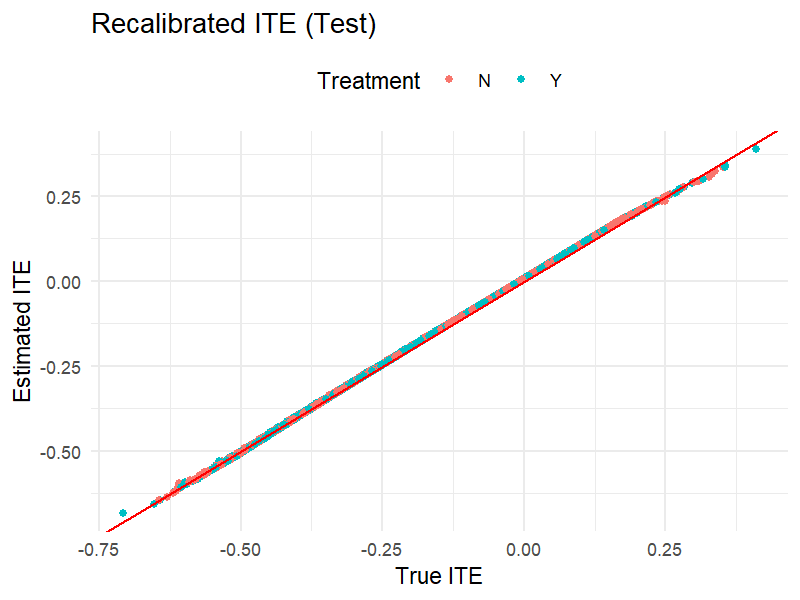
\includegraphics[width=0.7\linewidth]{img/ITE_recal.png}
% \vspace{0.8cm}
% 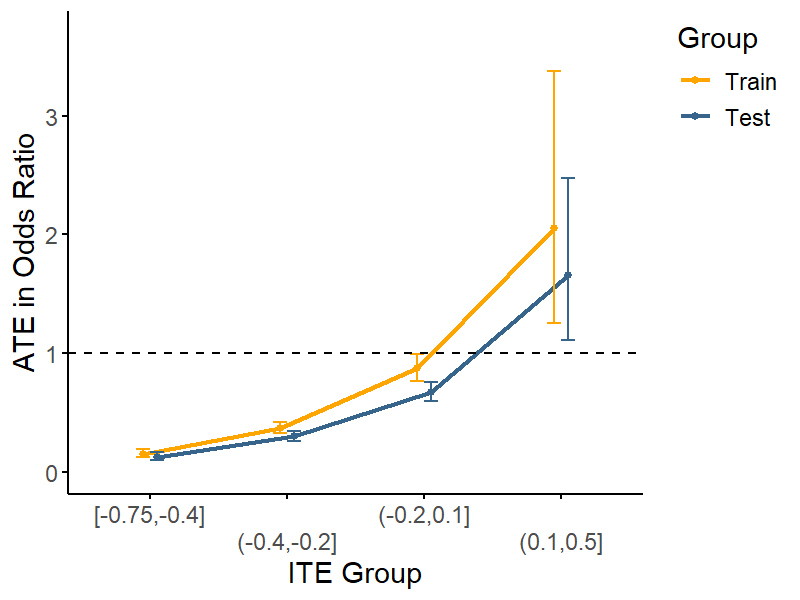
\includegraphics[width=0.7\linewidth]{img/ATE_ITE_recal.png}
% \end{column}
% \end{columns}
% 
% \end{frame}
% 
% 
% 
% % \begin{frame}{Background: The NISCI Study}
% 
% <<table1, echo=FALSE, results='hide' >>=
% 
% # # subset only baseline measures
% # visit_2 <- subset(datc, visit_id == 2)
% # 
% # ## Get variables names
% # #dput(names(visit_2))
% # 
% # ## Vector of variables to summarize
% # myVars <- c("uems","tissue_mid", "country")
% # 
% # # Create a TableOne object with an overall column
% # tab2 <- CreateTableOne(vars = myVars, strata = "trt", data = visit_2, addOverall = TRUE, test = FALSE)
% # 
% # # Convert TableOne to data frame for LaTeX formatting
% # tab2_df <- print(tab2, printToggle = FALSE, noSpaces = TRUE)
% # 
% # rownames(tab2_df) <- c("Patients", "UEMS (mean (SD))",  "Tissue Bridges (mean (SD))", "Country (%)", "Czech Republic", "Germany", "Spain", "Switzerland")
% # 
% # colnames(tab2_df) <- c("Overall", "Placebo", "NG101")
% # 
% # tab2_xt <- xtable(tab2_df, caption = "Baseline Characteristics by Treatment Group", label = "tab:table1")
% # 
% # # Print xtable
% # print(tab2_xt, include.rownames = TRUE, caption.placement = "top", type = "latex")
% 
% @
% 
% 
% % \end{frame}
% 
% 
% 
% 
% % \begin{frame}{Background: The NISCI Study}
% %     \centering
% %     \vspace{0.2cm}
% % <<figure_uems_tissue, echo=FALSE>>=
% % 
% % # quantiles <- quantile(subset(datc, visit_id==2)$SR, prob = 1:3/4, na.rm = TRUE)
% % # datc$SRc <- cut(datc$SR, breaks=c(-Inf, quantiles, Inf), as.ordered=TRUE)
% % 
% % # xyplot(uems ~ tm | trtplot , data = datc, group = id, xlim = c(-5, 240), type = "b", 
% % #        between = list(x = 1, y = 1), pch = 20, cex = .7,
% % #        lwd = 3, col = rgb(.1, .1, .1, .3), 
% % #        xlab = "Time (in days)",
% % # 			 ylab = "Upper Extremity Motor Score",
% % # 			 main = "Recovery in Upper Extremity Motor Score over time",
% % # 			 scales = list(
% % #          x = list(alternating = 1), # Show x-axis tick labels only at the bottom
% % #          tck = c(1, 0) # Remove top ticks
% % #        ),
% % #        )
% % 
% % 
% % @
% % \end{frame}
% % 
% 
% 
% % 
% % \begin{frame}{Methods: Generalized Additive Model (GAM)}
% % 
% % % Generalized additive models replace the linear form 
% % % $\sum \beta_j X_j$ by a sum of smooth functions $\sum f_j(X_j)$ \citep{hastie1986}.
% % 
% % %add vertical space
% % \vspace{5pt}
% % 
% % \begin{equation*}
% % \text{UEMS}_{ij} = \beta_0 + f_1(\text{tissue}_{i}) + f_2(\text{time}_{ij}) + f_3(\text{tissue}_{i}, \text{time}_{ij}) + b_{0i} + b_{1i} \cdot \text{time}_{ij} + \epsilon_{ij}
% % \end{equation*}
% % 
% % \textbf{Variables:} 
% % 
% % \begin{itemize}
% % \item UEMS: for individual $i$ at time $j$
% % \item Tissue: Parasagittal tissue bridges at baseline
% % \item Time: standardized (Time=0 corresponds to day of first medication and Time=1 is at 6-months follow up)
% % \item Random slope and intercept for each individual $i$
% % \item \(\epsilon_{ij} \sim \mathcal{N}(0, \sigma^2)\)
% % \end{itemize}
% % 
% % 
% % 
% % \end{frame}
% 
% 
% 
% % \begin{frame}{Results: Baseline Tissue Bridges}
% %     \centering
% %     \vspace{0.2cm}
% % <<figure_baseline_uems_tissue, echo=FALSE, error=FALSE, warning=FALSE, results='asis'>>=
% % # 
% % # xyplot(uems ~ SR | trtplot, 
% % #        data = subset(datc, visit_id == 2), 
% % #        group = id, 
% % #        type = "b", 
% % #        pch = 16,
% % #        cex = 1.2,
% % #        lwd = 2,
% % #        col = rgb(.1, .1, .1, .5),
% % #        xlab = "Parasagittal tissue bridges",
% % #        ylab = "Upper Extremity Motor Score",
% % #        main = "Baseline tissue bridges vs UEMS",
% % #        grid = TRUE,
% % # 			 scales = list(
% % #          x = list(alternating = 1), # Show x-axis tick labels only at the bottom
% % #          tck = c(1, 0) # Remove top ticks
% % #        ),
% % # 			 panel = function(x, y, ...) {
% % #          panel.xyplot(x, y, ...) # Plot the points
% % #          panel.lmline(x, y, col = "black", lwd = 1)  # Add a linear regression line
% % #        }
% % #        )
% % 
% % 
% % @
% % \end{frame}
% % 
% % 
% % 
% 
% 
% \begin{frame}{Outlook}
% 
% 
% \textbf{What we also did:}
% 
% \begin{itemize}
%     \item Ordinal predictors
%     \item TRAM-DAG on real climate data
% \end{itemize}
% 
% \vspace{0.4cm}
% 
% \textbf{What comes next:}
% \begin{itemize}
%     \item ITE estimation on real RCT-data
%     \item If time: include image data
% \end{itemize}
% 
% 
% \end{frame}
% 
% 


\begin{frame}{References}
  \small
  \bibliographystyle{apalike}
\bibliography{C:/Users/kraeh/OneDrive/Dokumente/Desktop/UZH_Biostatistik/Masterarbeit/MA_Mike/presentation_report/literature/bibSTA490}
\end{frame}

\end{document}
